%%%%%%%%%%%%%%%%%%%%%%%%%%%%%%%%%%%%%%%%%%%%%%%%%%%%%%%%%%%%%%%%%%%%%%%%%%%%%%%
% FILO-PRIORI - IEEE TRANSACTIONS ON SOFTWARE ENGINEERING
%%%%%%%%%%%%%%%%%%%%%%%%%%%%%%%%%%%%%%%%%%%%%%%%%%%%%%%%%%%%%%%%%%%%%%%%%%%%%%%
%
% Target: IEEE Transactions on Software Engineering (IEEE TSE)
% Template: IEEEtran (IEEE Computer Society Transactions)
%
% Structure:
%   - sections/introduction.tex
%   - sections/background.tex
%   - sections/related_work.tex
%   - sections/approach.tex
%   - sections/experimental_design.tex
%   - sections/results.tex
%   - sections/discussion.tex
%   - sections/threats.tex
%   - sections/conclusion.tex
%
%%%%%%%%%%%%%%%%%%%%%%%%%%%%%%%%%%%%%%%%%%%%%%%%%%%%%%%%%%%%%%%%%%%%%%%%%%%%%%%

\documentclass[10pt,journal,compsoc]{IEEEtran}

%------------------------------------------------------------------------------
% PACKAGES
%------------------------------------------------------------------------------
\usepackage{cite}
\usepackage{amsmath,amssymb,amsfonts}
\usepackage{algorithmic}
\usepackage{graphicx}
\usepackage{textcomp}
\usepackage{xcolor}
\usepackage{booktabs}
\usepackage{multirow}
\usepackage{array}
\usepackage{url}
\usepackage{hyperref}
\usepackage{balance}

% For code listings
\usepackage{listings}
\lstset{
  basicstyle=\footnotesize\ttfamily,
  breaklines=true,
  frame=single
}

% For subfigures — caption compatibility with IEEEtran
\usepackage[compatibility=false]{caption}
\usepackage{subcaption}

% For table notes
\usepackage{threeparttable}

% For colored boxes (findings summary)
\usepackage[most]{tcolorbox}

%------------------------------------------------------------------------------
% CUSTOM COMMANDS
%------------------------------------------------------------------------------
\newcommand{\filopriori}{\textsc{Filo-Priori}}
\newcommand{\apfd}{\textsc{APFD}}
\newcommand{\gatv}{GATv2}

% Highlight for revision
\newcommand{\todo}[1]{\textcolor{red}{[TODO: #1]}}
\newcommand{\rev}[1]{\textcolor{blue}{#1}}

%------------------------------------------------------------------------------
% DOCUMENT START
%------------------------------------------------------------------------------
\begin{document}

%------------------------------------------------------------------------------
% TITLE
%------------------------------------------------------------------------------
\title{Filo-Priori: Co-Failure Graph Attention for Test Case Prioritization in Continuous Integration}

%------------------------------------------------------------------------------
% AUTHORS
%------------------------------------------------------------------------------
\author{
  \IEEEauthorblockN{Acauan C. Ribeiro\IEEEauthorrefmark{1},
    Eduardo L. Feitosa\IEEEauthorrefmark{1},
    Andre L. da Costa Carvalho\IEEEauthorrefmark{1},\\
    Eulanda M. dos Santos\IEEEauthorrefmark{1},
    Bruno F. Gadelha\IEEEauthorrefmark{1},
    Yan R. Soares\IEEEauthorrefmark{1},
    and Jose Nascimento\IEEEauthorrefmark{2}}
  \IEEEauthorblockA{\IEEEauthorrefmark{1}Instituto de Computa\c{c}\~{a}o (IComp)\\
    Universidade Federal do Amazonas (UFAM)\\
    Manaus, AM, Brazil\\
    \{acauan.ribeiro, efeitosa, andre, emsantos, bruno, yan.soares\}@icomp.ufam.edu.br}
  \IEEEauthorblockA{\IEEEauthorrefmark{2}Motorola Mobility Com\'{e}rcio de Produtos Eletr\^{o}nicos Ltda.\\
    Manaus, AM, Brazil\\
    josern@motorola.com}
}

%------------------------------------------------------------------------------
% HEADERS
%------------------------------------------------------------------------------
\markboth{IEEE Transactions on Software Engineering, Vol. XX, No. X, Month 2026}%
{Ribeiro \MakeLowercase{\textit{et al.}}: Filo-Priori: Co-Failure Graph Attention for TCP in CI}

%------------------------------------------------------------------------------
% ABSTRACT
%------------------------------------------------------------------------------
\IEEEtitleabstractindextext{%
\begin{abstract}
In Continuous Integration (CI), growing test suites make exhaustive testing
impractical, motivating Test Case Prioritization (TCP) to maximize early
fault detection. Existing TCP approaches typically treat tests as independent
entities, ignoring structural relationships: tests that co-fail share
underlying dependencies, and execution patterns reveal systematic connections.
We present \filopriori{}, a graph-based deep learning framework for TCP that
models inter-test relationships through Graph Attention Networks (GATv2)
over a co-failure graph, complemented by a Deep Neural Network (DNN)
ensemble with data-driven blending for semantically-sparse settings. We
compare \filopriori{} with five baselines on two datasets: an industrial CI
pipeline (52,102 executions across 1,339 builds) and the RTPTorrent
benchmark (20 Java projects, 2,937 builds with failures). On the industrial
dataset, \filopriori{} achieves APFD~$=$~0.761 with significant improvements
over all five baselines ($+10.2\%$ to $+27.6\%$, $p < 0.001$). On RTPTorrent,
it achieves the highest numerical APFD of 0.854; after Holm-Bonferroni
correction, only gains over two baselines remain robust, indicating that
the advantage requires sufficient co-failure graph density. Ablation studies
show co-failure edges are the decisive component ($+17.0\%$ in isolation,
$p < 0.001$); supplementary edge types do not improve aggregate performance.
Two notable findings emerge: (1)~generic Sentence-BERT embeddings provide
no significant improvement ($p = 0.309$), confirmed by a Random-Fixed
control ($p = 0.965$); and (2)~\filopriori{}'s dual-balancing strategy is
not transferable to flat-feature architectures, confirming the gain is
structural. Temporal cross-validation and sensitivity analysis confirm
robustness across time periods and hyperparameter choices.
\end{abstract}

%------------------------------------------------------------------------------
% KEYWORDS
%------------------------------------------------------------------------------
\begin{IEEEkeywords}
Test Case Prioritization, Graph Attention Networks, Deep Learning,
Continuous Integration, Test Relationship Graph, Class Imbalance
\end{IEEEkeywords}
}

\maketitle

%------------------------------------------------------------------------------
% SECTION 1: INTRODUCTION
%------------------------------------------------------------------------------
\section{Introduction}
\label{sec:introduction}
\IEEEPARstart{C}{ontinuous} Integration (CI) has become a fundamental practice
in modern software development, enabling teams to integrate code changes frequently
and detect defects early~\cite{hilton2016usage, fowler2006continuous}. A key
challenge in CI environments is managing the growing test suite: as software
evolves, the number of test cases increases, making it impractical to execute
all tests for every commit~\cite{memon2017taming}.

Test Case Prioritization (TCP) addresses this challenge by ordering test cases
to maximize early fault detection~\cite{rothermel2001prioritizing, elbaum2002test}.
The goal is to execute tests most likely to fail first, providing faster feedback
to developers. The effectiveness of TCP is typically measured using the Average
Percentage of Faults Detected (APFD) metric~\cite{rothermel1999test}.

However, existing TCP approaches, whether based
on coverage~\cite{rothermel2001prioritizing}, historical failure~\cite{kim2002history},
or machine learning~\cite{spieker2017reinforcement, pan2022test}, often treat
test cases as independent entities. This assumption ignores the rich relationships
inherent in test suites: tests that co-fail in the same build often share underlying dependencies,
tests with similar descriptions target related functionality, and historical execution patterns
frequently reveal systematic structural connections~\cite{german2009evolution}.

Hence, our key insight is that \emph{structural patterns}, particularly failure
co-occurrence modeled through graph neural networks, provide a fundamental source of information
for TCP. Initially, we hypothesized that semantic information (test descriptions,
commit messages) would provide a complementary source. However, this work shows
that generic pre-trained sentence-level embeddings
(Sentence-BERT) yield no statistically significant improvement when
structural features and graph-based propagation are available. This
result challenges the assumption that off-the-shelf semantic similarity is a
strong predictor of failure~\cite{hernandes2025method}, and constitutes a
key finding of this work: \emph{how tests have behaved} is more predictive
than \emph{what generic sentence embeddings capture from test
descriptions}. We emphasize that this finding applies specifically to
pre-trained, domain-agnostic sentence encoders. Code-aware language models
(e.g., CodeBERT~\cite{feng2020codebert}, StarCoder), AST-based
representations, or models fine-tuned on software engineering corpora may
extract relevant features that generic embeddings miss, and remain an open
research direction.

Considering this context, we present
\filopriori{}, a graph-based framework for TCP with three architectural
components:

\begin{enumerate}
    \item \textbf{GATv2 over a Co-Failure Test Relationship Graph}: We model
    test case relationships through a graph where nodes are test cases and
    co-failure edges encode behavioral co-occurrence.
    GATv2~\cite{brody2022attentive} propagates failure information between related
    tests with learned attention weights. Co-failure edges, universally
    available from CI logs, are the core graph type and provide sufficient
    information for effective prioritization. When richer metadata exists, the
    graph can optionally extend to a multi-edge configuration with up to five
    complementary edge types. The per-edge-type
    ablation (Section~\ref{sec:rq2}) provided in this work shows that co-failure alone is optimal on the
    evaluated datasets.

    \item \textbf{DNN Ensemble with Data-Driven Blending}: The GNN predictions
    are complemented by a DeepOrder-inspired DNN~\cite{chen2023deeporder}
    predictor that scores tests based on per-test temporal features without
    requiring graph membership. A validation-optimized blending coefficient
    $\alpha$ combines the two predictors, naturally favoring the GNN when
    metadata is rich and the DNN when metadata is sparse.

    \item \textbf{Optional Semantic Stream}: The architecture includes
    a semantic stream (Sentence-BERT embeddings with cross-attention fusion)
    to explore whether textual metadata improves prioritization.
    As detailed in Section~\ref{sec:rq2}, this stream provides no
    statistically significant benefit, suggesting that co-failure graph
    modeling subsumes the discriminative signal that generic embeddings
    capture.
\end{enumerate}

Additionally, the training strategy addresses the severe class imbalance
typical of TCP data (up to 37:1 Pass:Fail ratio) through a simplified
dual-balancing approach: balanced sampling corrects the class prior at the
data level, while Focal Loss~\cite{lin2017focal} concentrates gradients on
hard-to-classify examples at the loss level
(Section~\ref{sec:training}).

We evaluate \filopriori{} on two complementary datasets: (1) an industrial
CI pipeline for mobile devices comprising 52,102 test executions
distributed across 1,339 builds (277 with failures) from a single
commercial project, where a build represents a complete cycle of code
integration and automated testing; and (2) the RTPTorrent benchmark with
20 open-source Java projects totaling over 100,000 Travis CI builds
(2,937 with failures). Our evaluation addresses four research questions:

\begin{itemize}
    \item \textbf{RQ1}: Can modeling structural relationships between test cases
    through graph neural networks improve fault detection compared to approaches
    that treat tests independently?
    \item \textbf{RQ2}: Which architectural components contribute most to the
    effectiveness of graph-based test case prioritization?
    \item \textbf{RQ3}: How robust is the proposed approach when applied to builds
    from different time periods than those used for training?
    \item \textbf{RQ4}: How sensitive is the approach to the choice of key
    hyperparameters?
\end{itemize}

Our results reveal that co-failure graph modeling is the primary
architectural factor. On the industrial dataset, \filopriori{} achieves an
APFD of 0.7611 with statistically significant improvements over all five
deep learning baselines ($+10.2\%$ to $+27.6\%$, $p < 0.001$); a
controlled experiment confirms this advantage is primarily architectural
(Table~\ref{tab:deeporder_dualbalancing}). On RTPTorrent, where co-failure
graph density is lower, \filopriori{} achieves the highest numerical APFD
of 0.8540 across 20 projects. However, after Holm-Bonferroni correction
only the improvements over NodeRank and RETECS are statistically robust,
while the margins over TCP-Net, FailRank-BB, and DeepOrder constitute a
statistical tie ($n=20$ projects).
Ablation studies reveal complementary patterns across the two variants:
on the industrial dataset, the GATv2 graph attention is the most critical
component (+17.0\%); on RTPTorrent, the DNN ensemble is the primary
contributor, though the execution-level temporal GNN substantially reduces
reliance on it (drop without DNN is only 2.6\%).

Therefore, this paper makes the following contributions:
\begin{enumerate}
    \item \textbf{Architectural}: An adaptive graph-based pipeline for TCP
    centered on GATv2 over a co-failure test relationship graph, with a
    DeepOrder-inspired~\cite{chen2023deeporder} DNN ensemble for metadata-sparse settings
    (Section~\ref{sec:ensemble}). Co-failure edges alone are sufficient;
    supplementary edge types are optional.
    \item \textbf{Negative result on semantic features}: Generic
    Sentence-BERT embeddings provide no significant improvement
    ($p = 0.309$) when structural features and co-failure propagation are
    available. A controlled experiment shows that when semantic baselines
    appear competitive, they exploit embeddings as identity proxies, not
    semantic content (Section~\ref{sec:rq1_rtptorrent}).
    \item \textbf{Empirical}: Evaluation against five baselines on two
    datasets: significant improvements on the industrial dataset
    ($+10.2\%$ to $+27.6\%$, $p < 0.001$), highest numerical APFD on
    RTPTorrent with robust gains over NodeRank and RETECS after
    Holm-Bonferroni correction. A controlled experiment confirms the
    advantage is primarily architectural, not from the class-imbalance
    strategy (Section~\ref{sec:rq1}).
    \item \textbf{Insights}: Actionable guidelines from ablation,
    sensitivity, and temporal validation: co-failure graphs are the
    decisive component; shallow GNNs (1~layer, 2~heads) suffice; and
    dual-balancing (sampling + focal loss) prevents mode collapse. A
    replication package is publicly available.
\end{enumerate}

\textbf{Paper Organization.} The remainder of this paper is organized as follows.
Section~\ref{sec:background} presents the fundamental background concepts that
underlie our approach.
Section~\ref{sec:related} discusses related work on TCP, reviewing traditional,
machine learning-based, and graph-based approaches.
Section~\ref{sec:approach} describes the \filopriori{} approach in detail,
including its graph-based architecture, feature extraction, graph construction,
and training strategy.
Section~\ref{sec:experimental} presents the experimental design.
Section~\ref{sec:results} reports the experimental results organized by
research questions.
Section~\ref{sec:discussion} discusses the implications of our findings
and the practical considerations for adopting \filopriori{}.
Section~\ref{sec:threats} addresses threats to the validity of our study.
Finally, Section~\ref{sec:conclusion} concludes the paper and outlines
directions for future work.

%------------------------------------------------------------------------------
% SECTION 2: BACKGROUND
%------------------------------------------------------------------------------
\section{Background}
\label{sec:background}

This section introduces fundamental concepts underlying our approach.

\subsection{Test Case Prioritization}
\label{sec:bg_tcp}

Test Case Prioritization (TCP) is the process of ordering test cases for execution
to achieve certain objectives, such as maximizing early fault detection~\cite{rothermel2001prioritizing}.
Formally, given a test suite $T$ and a permutation function $PT$ that produces
ordered sequences of $T$, TCP aims to find an ordering $T' \in PT$ that
maximizes a given objective function~\cite{elbaum2002test}.

In Continuous Integration environments, TCP is particularly important because:
(1) test suites grow over time, making exhaustive testing impractical~\cite{memon2017taming};
(2) developers need rapid feedback on code changes~\cite{hilton2016usage}; and
(3) computing resources for testing are often limited~\cite{spieker2017reinforcement}.

To illustrate the impact of effective prioritization, consider a test suite with
100 test cases where only 3 detect faults. Under random ordering, developers may
need to execute 50 or more tests before encountering a failure. An effective
prioritization strategy would place these 3 failing tests near the beginning of
the execution order, providing faster feedback and enabling developers to begin
debugging sooner.

\subsection{APFD Metric}
\label{sec:bg_apfd}

To quantify the effectiveness of a prioritization strategy, the research
community has adopted standardized metrics. The most widely used is the
Average Percentage of Faults Detected (APFD)~\cite{rothermel1999test}. For a test suite $T$
containing $n$ test cases that detect $m$ faults, with $TF_i$ being the position
of the first test case that detects fault $i$, APFD is calculated as:

\begin{equation}
    \text{APFD} = 1 - \frac{\sum_{i=1}^{m} TF_i}{n \times m} + \frac{1}{2n}
\end{equation}

It ranges from 0 to 1, where higher values indicate better prioritization.
An APFD of 0.5 corresponds to random ordering, while 1.0 indicates
prioritization where all faults are detected by the first tests.

\subsection{Graph Neural Networks and Graph Attention}
\label{sec:bg_gnn}

Graph Neural Networks (GNNs) are a class of deep learning models designed to
operate on graph-structured data~\cite{wu2021comprehensive}. The core principle
underlying GNNs is \emph{message passing}: each node updates its representation
by aggregating information from its neighbors, enabling the model to capture
structural patterns in the graph topology. Formally, a GNN layer computes:
\begin{equation}
    h_i^{(l+1)} = \text{UPD}\!\left(h_i^{(l)},\; \text{AGG}\!\left(\{h_j^{(l)} : j \in \mathcal{N}(i)\}\right)\right)
\end{equation}
where $h_i^{(l)}$ is the representation of node $i$ at layer $l$, $\mathcal{N}(i)$
is the set of neighbors of node $i$, and UPDATE and AGGREGATE are learnable functions.

Several GNN variants differ in how they implement these functions.
Graph Convolutional Networks (GCN)~\cite{kipf2017semi} use normalized adjacency
for aggregation, GraphSAGE~\cite{hamilton2017inductive} samples and aggregates
from local neighborhoods, and Graph Attention Networks
(GAT)~\cite{velickovic2018graph} introduce learned attention mechanisms to
weigh neighbor contributions. Brody et al.~\cite{brody2022attentive} showed
that standard GAT computes a restricted form of ``static'' attention where
the ranking of attention scores is independent of the query node, and proposed
GATv2, which applies the nonlinearity \emph{after} the linear transformation:
\begin{equation}
    \alpha_{ij} = \text{softmax}_j\left(\vec{a}^T \cdot \text{LeakyReLU}\left(\mathbf{W}[\vec{h}_i \| \vec{h}_j]\right)\right)
\end{equation}
This modification enables ``dynamic'' attention where attention scores depend
on both the query and key nodes, providing higher expressiveness. In this
work, we adopt GATv2 due to its ability to learn the relative importance of
different neighbors, which is relevant for TCP where different types of test
relationships (e.g., co-failure vs.\ semantic similarity) carry different
predictive value. Section~\ref{sec:fusion} presents the specific architectural
configuration and its interaction with the test relationship graph.

\subsection{Class Imbalance and Focal Loss}
\label{sec:bg_focal}

Test execution data typically exhibits severe class imbalance, with far more
passing tests than failing tests~\cite{spieker2017reinforcement, chen2023deeporder}.
Standard cross-entropy loss is dominated by the majority class, leading to models
that predict ``pass'' for nearly all tests.

\textbf{Focal Loss}~\cite{lin2017focal} addresses this by down-weighting easy
examples and focusing on hard ones:

\begin{equation}
    \text{FL}(p_t) = -\alpha_t (1 - p_t)^\gamma \log(p_t)
\end{equation}

where $p_t$ is the predicted probability of the true class, $\alpha_t$ is a
class-balancing weight, and $\gamma$ is the focusing parameter. When $\gamma > 0$,
the $(1 - p_t)^\gamma$ term reduces the loss for well-classified examples,
focusing training on hard negatives.

\subsection{Cross-Attention Mechanisms}
\label{sec:bg_cross_attn}

Cross-attention~\cite{vaswani2017attention} extends the self-attention paradigm
to the \emph{inter-modal} setting: one representation (the \emph{query})
selectively attends to a second representation (the \emph{key/value}),
enabling information exchange across heterogeneous feature spaces. Concretely,
given a query matrix $Q \in \mathbb{R}^{n \times d_k}$ drawn from one modality
and key/value matrices $K, V \in \mathbb{R}^{m \times d_k}$ drawn from another,
cross-attention computes:

\begin{equation}
    \text{CrossAttn}(Q, K, V) = \text{softmax}\left(\frac{QK^T}{\sqrt{d_k}}\right)V
\end{equation}

\noindent
Each row of the output is a weighted combination of the value vectors,
where the weights are determined by the compatibility (dot-product similarity)
between the corresponding query and all keys, scaled by $\sqrt{d_k}$ to
prevent gradient saturation. When applied bidirectionally (each modality
serves as both query and key/value in turn), the mechanism allows both
representations to be enriched with complementary information from the other.

In \filopriori{}, we apply bidirectional cross-attention to fuse structural
features (derived from the GATv2 graph stream) with semantic features
(derived from Sentence-BERT embeddings). The architectural motivation is
twofold: (1) cross-attention can, in principle, discover fine-grained
correlations between textual content and behavioral patterns (e.g., a test
whose description mentions a specific module might attend to the failure
signal of structurally related tests); and (2) unlike simple concatenation,
cross-attention preserves the dimensionality of each stream through residual
connections, avoiding the dilution that occurs when high-dimensional
semantic vectors dominate the fused representation.

As shown in Section~\ref{sec:rq2}, cross-attention does not yield a
statistically significant improvement in the evaluated settings, indicating
that the semantic stream carries insufficient discriminative signal for the
fusion mechanism to exploit. We retain cross-attention in the architecture
because it imposes negligible computational overhead and is the standard
mechanism for multi-modal fusion~\cite{vaswani2017attention,
wu2021comprehensive}. Future deployments with domain-specific embeddings
(e.g., code-aware language models) may produce stronger textual signals.

%------------------------------------------------------------------------------
% SECTION 3: RELATED WORK
%------------------------------------------------------------------------------
\section{Related Work}
\label{sec:related}

This section reviews prior work on TCP. We organize related work into three
groups reflecting the evolution of TCP methods: (1) traditional and coverage-based
approaches, which rely on code structure and execution information;
(2) shallow and deep learning approaches, which learn prioritization
patterns from historical data; and (3) graph-based approaches, which explicitly
model relationships between test artifacts. Each group represents a different
strategy for capturing the information needed for effective prioritization.

\subsection{Traditional and Coverage-based TCP}

Early TCP research focused on code coverage-based techniques.
Rothermel et al.~\cite{rothermel2001prioritizing} proposed total and additional
coverage prioritization strategies, where test cases are ordered based on the
number of code statements or branches they cover.
Li et al.~\cite{li2007search} demonstrated the effectiveness of search-based
approaches for TCP, exploring genetic algorithms for optimizing test orderings.
Walcott et al.~\cite{walcott2006timeaware} proposed time-aware TCP techniques
that consider both coverage and execution cost.
The advantage of coverage-based approaches is their strong theoretical foundation
and direct connection to code structure. However, they require instrumentation
and access to source code, which limits their applicability in black-box testing
scenarios.
Elbaum et al.~\cite{elbaum2002test} conducted extensive empirical studies comparing
coverage-based strategies, showing that the effectiveness of different techniques
varies significantly across programs and versions, and that no single strategy
dominates in all scenarios.
Henard et al.~\cite{henard2016comparing} compared white-box and black-box TCP
techniques at scale, finding that similarity-based approaches can be competitive
with coverage-based methods while requiring less instrumentation.
History-based approaches leverage past test execution results.
Kim and Porter~\cite{kim2002history} showed that tests that failed
recently are more likely to fail again, a simple yet effective heuristic.
The main advantage of history-based methods is their low computational cost and
independence from source code. Their limitation is the inability to handle new
test cases or tests that have not yet failed.

\subsection{Machine Learning-Based Approaches}

Machine learning has been increasingly applied to TCP, aiming to learn complex
patterns from historical execution data.
Spieker et al.~\cite{spieker2017reinforcement} introduced RETECS
(Reinforcement learning for automatic Test Case prioritization and Selection
in Continuous Integration), a pioneering approach that frames TCP as a
reinforcement learning problem. RETECS treats each CI cycle as an episode
and learns to prioritize tests by maximizing a reward signal based on fault
detection. Its advantage is the ability to continuously adapt to changing test
patterns without retraining. However, it requires a significant number of CI
cycles to converge and may struggle with sparse failure signals.

Chen et al.~\cite{chen2023deeporder} proposed DeepOrder, a deep learning approach
for TCP in continuous integration testing. DeepOrder uses a deep neural network
that takes as input eight historical features per test case (including last
execution result, time since last failure, and failure rate) to predict the
likelihood of failure. The predicted probabilities are then used to rank test cases.
DeepOrder demonstrated improvements over simple heuristics. However, it treats
test cases independently without considering relationships between them, and it
relies solely on historical features without incorporating semantic information
from test descriptions or commit messages.

TCP-Net~\cite{abdelkarim2022tcp} introduced an end-to-end deep learning approach
that learns directly from test execution data, aiming to capture temporal patterns
in test execution sequences. While it showed promising results, it also treats
tests as independent entities and does not model structural relationships.

Busjaeger and Xie~\cite{busjaeger2016learning} proposed a learning-to-rank approach
for TCP that combines multiple information sources (code coverage, text similarity,
and historical data) into a unified ranking model, demonstrating the value of
multi-source feature integration.
Bagherzadeh et al.~\cite{bagherzadeh2022reinforcement} conducted a comprehensive
study of reinforcement learning (RL) approaches for TCP, finding that while RL methods
can adapt to changing environments, they often require substantial training data
to converge.
Bertolino et al.~\cite{bertolino2020learning} explored learning-based TCP in
industrial CI settings, identifying challenges such as test suite evolution and
flaky tests that affect practical deployment.
Pan et al.~\cite{pan2022test} proposed a test case prioritization approach that
combines multiple information sources using attention mechanisms, demonstrating
improvements over single-feature approaches.

Hernandes et al.~\cite{hernandes2025method} proposed a method for ordering
regression testing plans in the context of non-automated, black-box testing.
Their approach uses Sentence-BERT to extract embeddings from test case scripts
and commit messages, then employs machine learning classifiers (KNN, Logistic
Regression, MLP, XGBoost, Random Forest) to predict the failure probability of
each test case. Test cases are then ordered by their predicted failure probability.
Their experiments showed results equal to or better than human experts in
92.52\% to 94.24\% of scenarios. While this work demonstrated the value of
semantic information from test descriptions and commits for TCP, it does not
model structural relationships between test cases and relies on traditional
machine learning classifiers rather than graph-based architectures. \filopriori{}
builds upon this work by incorporating structural features and graph-based
learning to capture test relationships.

\subsection{Graph-Based Approaches}

Li et al.~\cite{li2024noderank} proposed NodeRank, a test input prioritization
approach for GNNs using mutation-based analysis. NodeRank leverages ensemble
learning-based ranking models (including LightGBM and Random Forest) with three
types of mutations: graph structure mutations (edge additions/removals), node
feature mutations (Gaussian noise injection), and model mutations (weight
perturbation). For each test input (graph node), NodeRank computes a priority score
based on how sensitively the model's prediction changes under these mutations.
NodeRank was evaluated on Cora, CiteSeer, and PubMed citation network datasets,
outperforming uncertainty-based baselines
by significant margins. While NodeRank was originally designed for GNN model
testing rather than software TCP, we include it as a baseline because its
core mechanism (ensemble-based ranking from structural graph
features) is directly applicable to TCP when the ``GNN under test'' is
replaced with a test relationship graph and mutations are applied to test
execution features rather than citation network inputs. In our adaptation,
NodeRank's graph structure mutations correspond to perturbations of the
co-failure graph, and its node feature mutations inject noise into the
structural features used by all methods. This adaptation is faithful to
NodeRank's published algorithm; its core noise injection mechanics perturb
adjacency matrices and feature vectors mathematically, remaining entirely
agnostic to whether the original edges represent paper citations or test
co-failures. A key limitation is its reliance on mutation-based
analysis, which requires running the model multiple times per test input,
increasing computational cost.

\subsection{Summary and Positioning of \filopriori{}}

The reviewed literature gaps that \filopriori{} aims to address.
Traditional coverage-based approaches require source code access and cannot
capture complex inter-test relationships. Deep learning approaches
(RETECS, DeepOrder, TCP-Net) have demonstrated the value of learning from
historical data, but they treat test cases independently, missing structural
dependencies. FailRank-BB~\cite{hernandes2025method} demonstrated the value of
semantic information from test descriptions and commits, but relies on
traditional classifiers (Logistic Regression) without modeling inter-test
relationships. Graph-based approaches (NodeRank) have shown the potential of
modeling relationships, but focus on GNN model testing rather than software TCP.
Table~\ref{tab:rw_positioning} summarizes the key differences between
\filopriori{} and the five deep learning baselines used in our evaluation.

\begin{table}[!t]
\centering
\caption{Positioning of \filopriori{} against deep learning baselines.}
\label{tab:rw_positioning}
\footnotesize
\resizebox{\columnwidth}{!}{%
\begin{tabular}{lccccc}
\toprule
\textbf{Method} & \textbf{Semantic} & \textbf{Structural} & \textbf{Graph} & \textbf{Cross-Attn} & \textbf{Orphan} \\
\midrule
DeepOrder & -- & \checkmark & -- & -- & -- \\
TCP-Net & -- & \checkmark & -- & -- & -- \\
NodeRank & -- & \checkmark & \checkmark & -- & -- \\
RETECS & -- & \checkmark & -- & -- & -- \\
FailRank-BB & \checkmark & -- & -- & -- & -- \\
\midrule
\textbf{\filopriori{}} & \checkmark & \checkmark & \checkmark & \checkmark & \checkmark \\
\bottomrule
\end{tabular}%
}
\end{table}

\filopriori{} distinguishes itself from these approaches primarily through:
(1) explicitly modeling test case co-failure relationships through a graph
where GATv2~\cite{brody2022attentive} propagates failure signals with
dynamic attention, enabling the model to capture structural dependencies
that flat-feature approaches miss; (2) a configurable scoring pipeline
(GNN-only or GNN+DNN ensemble) with validation-optimized blending that
adapts to the available metadata; and (3) co-failure edges as the core
graph component, requiring only CI execution logs for deployment.
The architecture also includes supplementary edge types and a
semantic stream (Table~\ref{tab:rw_positioning}).
We evaluate \filopriori{} on two complementary datasets spanning industrial
TCP and open-source projects to assess generalization across domains.

%------------------------------------------------------------------------------
% SECTION 4: APPROACH
%------------------------------------------------------------------------------
\section{Approach: \filopriori{}}
\label{sec:approach}

This section describes the \filopriori{} approach for Test Case Prioritization.

\subsection{Overview}

The \filopriori{} architecture takes as input: (1) historical test execution
patterns (structural features); (2) a co-failure test relationship graph
(with optional multi-edge extensions when metadata permits); and
(3) optionally, text embeddings of test descriptions and commit messages. It
outputs a ranking of test cases by predicted failure probability.
Figure~\ref{fig:framework} presents an overview of the framework.

The core architecture centers on two predictive components:
\begin{enumerate}
    \item \textbf{GATv2 Structural Stream}: A Graph Attention Network that
    processes historical features over the co-failure test relationship
    graph, learning to propagate failure signals between related tests
    through learned attention weights. As shown in Section~\ref{sec:rq2},
    this is the dominant contributor to prioritization effectiveness, and
    co-failure edges are sufficient for effective prioritization.
    \item \textbf{DNN Ensemble}: A DeepOrder-inspired feedforward network that
    scores tests based on per-test temporal features without requiring graph
    membership. When combined with the GNN through validation-optimized
    blending, it provides complementary signal in settings where graph
    structure alone is insufficient (Section~\ref{sec:ensemble}).
\end{enumerate}

The architecture additionally includes a \textbf{semantic stream}
and a \textbf{cross-attention fusion} module that combines semantic and
structural representations. We included these components to test whether
textual metadata improves prioritization. As detailed in
Section~\ref{sec:rq2}, they do not provide a statistically significant
improvement in the evaluated settings, yielding a valuable negative result
discussed in Section~\ref{sec:discussion}.

\filopriori{} is a single adaptive pipeline whose active components are
determined by the available metadata, not by manual architectural selection.
Table~\ref{tab:rtptorrent_config} summarizes the two deployment
configurations evaluated in this work:
\begin{itemize}
    \item \textbf{\textsc{Filo-Priori-Full}} (metadata-rich setting): The
    pipeline constructs a co-failure graph as the core. When rich metadata
    is available (test descriptions, commit messages, component labels,
    scheduling data), supplementary edge types can optionally be
    activated. The per-edge-type ablation (Section~\ref{sec:rq2}) shows that
    co-failure edges alone provide optimal performance. A KNN orphan
    pipeline handles test cases absent from the training graph. The GNN
    probability is the final prioritization score, as the
    validation-optimized $\alpha$-blending naturally assigns full weight
    to the GNN.
    \item \textbf{\textsc{Filo-Priori-Ensemble}} (metadata-sparse setting):
    When metadata is limited to test names and CI logs, the pipeline
    degrades smoothly: only co-failure edges are constructed (the
    remaining edge types produce no edges due to absent metadata), and the
    DNN ensemble activates as a complementary scoring channel. The
    validation-optimized $\alpha$-blending coefficient automatically
    balances the GNN and DNN based on their relative effectiveness for
    each project.
\end{itemize}
Both configurations share the same core architecture (feature engineering,
GATv2 graph model, training strategy, DNN ensemble, $\alpha$-blending). They
differ only in which modules are \emph{activated} by the available data.
The graph construction uses only the edge types supported by the metadata
(Section~\ref{sec:graph}), and the $\alpha$-blending selects the scoring
balance automatically (Section~\ref{sec:ensemble}). In practice, the only
human decision is which textual fields to encode; the rest adapts to the
deployment context.

The remainder of this section describes the shared components
(Sections~\ref{sec:feature_engineering}--\ref{sec:fusion}), the training
strategy (Section~\ref{sec:training}), and the deployment-specific extensions
(Section~\ref{sec:deployment}).

\begin{figure}[!t]
    \centering
    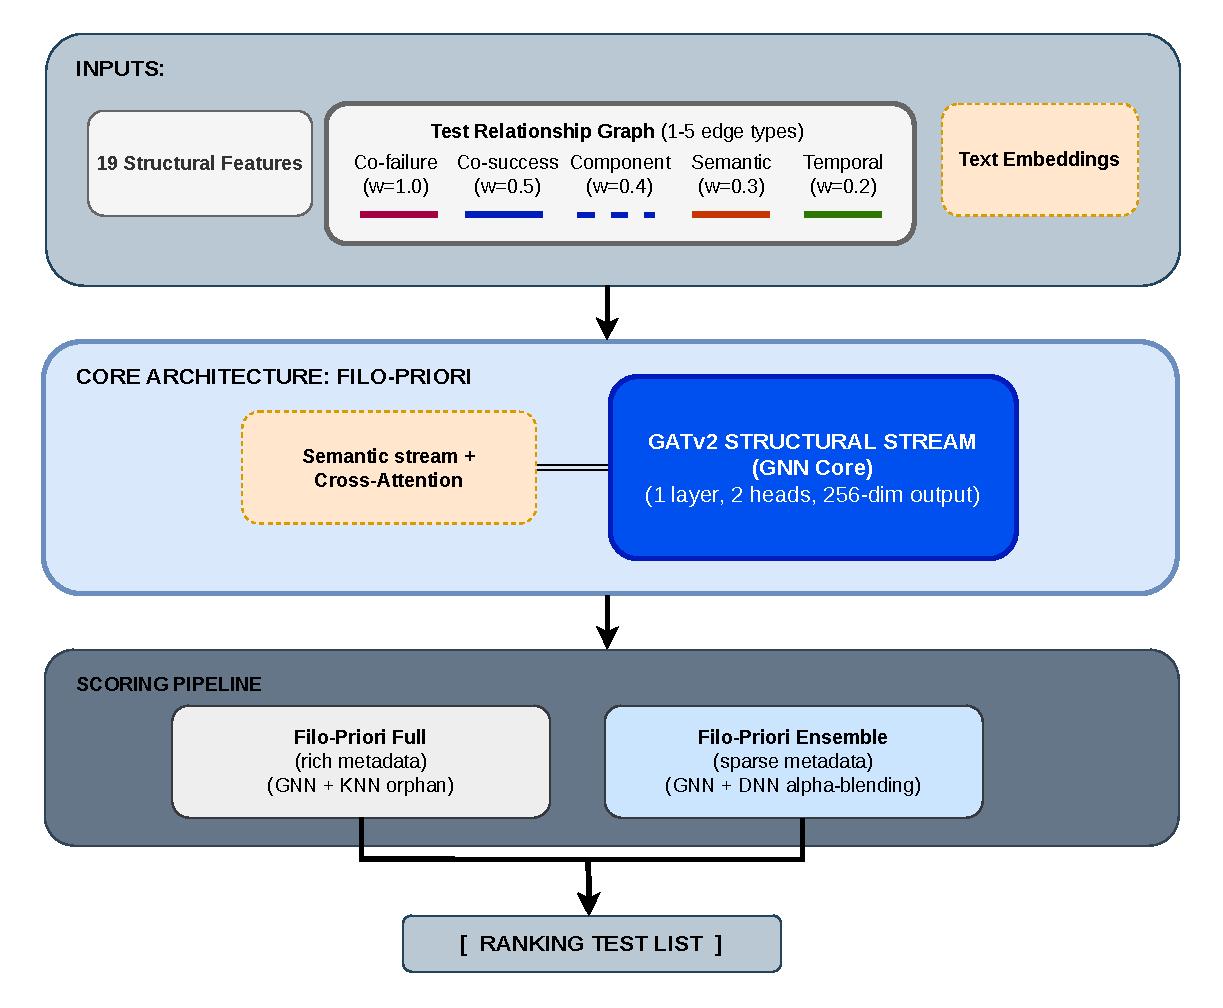
\includegraphics[width=\columnwidth]{figures/filo-priori-overview.pdf}
    \caption{Overview of the \filopriori{} framework. The core architecture
    centers on the GATv2 structural stream operating over the
    co-failure test relationship graph, complemented by a DNN ensemble with
    data-driven blending. Co-failure edges are the dominant graph component
    (Section~\ref{sec:rq2}); supplementary edge types and the semantic
    stream (dashed) are optional extensions that do not improve aggregate
    performance on the evaluated datasets. Not all components are active in
    every deployment configuration (see Table~\ref{tab:rtptorrent_config}).}
    \label{fig:framework}
\end{figure}

\subsection{Feature Engineering}
\label{sec:feature_engineering}

\filopriori{} combines two complementary feature types: semantic embeddings
that capture textual content, and structural features that capture historical
execution patterns.

\textbf{Semantic Features.}
We use Sentence-BERT~\cite{reimers2019sentence} with the
\texttt{all-mpnet-base-v2} model to encode available textual metadata into
768-dimensional embeddings. The semantic input depends on the metadata
available in each deployment context:

\emph{When rich metadata is available} (e.g., industrial test management
systems), we encode four textual fields per test case: the test case summary
(TC\_Summary), the detailed test steps (TC\_Steps), the commit message
associated with the code change, and the code diff (truncated to 2,000
characters). These four fields are aggregated into two
768-dimensional Sentence-BERT embeddings: the \emph{test case embedding}
combines TC\_Summary and TC\_Steps into a single description text encoded
by Sentence-BERT, while the \emph{commit embedding} combines the commit
message and the code diff into a single code-change text encoded by
Sentence-BERT. The two 768-dimensional embeddings are then concatenated
to form 1,536-dimensional semantic features, enabling the model to capture
relationships between test descriptions and code changes.

\emph{When metadata is sparse} (e.g., open-source CI systems), only test
class and method names are available. These are tokenized using camelCase
splitting and encoded into 768-dimensional embeddings. While less informative
than full descriptions, these embeddings still capture naming conventions that
reflect functional groupings.

The semantic stream architecture is agnostic to the input dimensionality.
Only the input projection layer adapts to the embedding size.

\textbf{Structural Features.}

We investigated a total of 29 candidate structural features capturing historical
execution patterns. These features were identified through a combination of
domain knowledge from the TCP literature~\cite{chen2023deeporder, kim2002history}
and analysis of the available execution data. After feature selection,
19 features were retained, organized into two categories.

\textbf{Base Features (10 features):} These features capture the fundamental
historical behavior of each test case:
\begin{itemize}
    \item \textbf{test\_age}: Number of builds since the test case first appeared
    in the execution history, indicating its maturity.
    \item \textbf{failure\_rate}: The ratio of failed executions to total
    executions across the entire history of the test case.
    \item \textbf{recent\_failure\_rate}: Failure rate computed over the last
    5 builds. We chose a window of 5 builds as it balances recency with
    statistical stability, following common practice in TCP
    literature~\cite{chen2023deeporder}.
    \item \textbf{flakiness\_rate}: The frequency of Pass$\leftrightarrow$Fail
    oscillations, computed as the number of status transitions divided by the
    total number of executions. Elevated oscillation rates may reflect
    sensitivity to code changes, environmental variability, or coupling with
    frequently modified modules. This feature captures the degree of
    behavioral instability regardless of its underlying cause.
    \item \textbf{consecutive\_failures}: The length of the current consecutive
    failure streak, capturing ongoing instability.
    \item \textbf{max\_consecutive\_failures}: The maximum consecutive failure
    streak observed in the test's history, indicating its worst-case behavior.
    \item \textbf{failure\_trend}: The difference between recent failure rate
    and overall failure rate, where positive values indicate deteriorating
    performance.
    \item \textbf{commit\_count}: Number of unique commits associated with
    the test case's execution history, reflecting code change activity.
    \item \textbf{cr\_count}: Number of distinct change requests (CRs)
    associated with the test, indicating the breadth of modifications.
    \item \textbf{test\_novelty}: A binary indicator (1 if the test case
    appears for the first time in the current build, 0 otherwise).
\end{itemize}

\textbf{DeepOrder-Inspired Features (9 features):} Following the temporal
feature engineering approach of DeepOrder~\cite{chen2023deeporder}, we added
features that capture recent execution dynamics. The
\textbf{execution\_status\_last\_$N$} features (for $N \in \{1, 2, 3, 5, 10\}$)
represent the proportion of failures in the last $N$ executions, providing
multi-scale windows that capture both immediate ($N{=}1$) and short-term
($N{=}10$) failure patterns. Additionally, we include
\textbf{cycles\_since\_last\_fail} (number of builds since the last failure,
normalized to $[0, 1]$), \textbf{distance} (temporal distance from the last
failure in calendar time, normalized), \textbf{status\_changes} (total number
of Pass$\leftrightarrow$Fail transitions, capturing behavioral instability),
and \textbf{fail\_rate\_last\_10} (failure rate over the last 10 executions,
complementing the 5-build window).

These temporal features capture patterns that static metrics miss: a test that
failed in the last execution is more likely to fail again than one that failed
only in distant history.

\textbf{Feature Selection.} We initially extracted 29 candidate features.
To reduce noise and improve generalization, we performed feature selection using
a two-step process: (1) importance analysis using a preliminary Random Forest
classifier to rank features by their contribution to failure prediction, and
(2) correlation filtering to remove redundant features with Pearson correlation
above 0.90. This process reduced the feature set from 29 to the 19 features
described above, retaining only those with meaningful discriminative power.
The selection was performed on the industrial training set (temporally
preceding the validation and test sets) without cross-validating the selection
process itself. Nonetheless, we acknowledge
that per-project feature selection on RTPTorrent could further improve
results by adapting to project-specific failure distributions, and we
identify this as a potential enhancement in future work.

\subsection{Test Relationship Graph Construction}
\label{sec:graph}

We construct a test relationship graph where nodes represent test cases and
edges capture behavioral relationships between them. The graph serves as the
backbone for GAT message passing, enabling failure signal propagation
between related tests.

\textbf{Co-failure edges (core).} The graph is built on co-failure edges,
which are universally available in any CI system with test execution logs
and carry the strongest predictive signal for related test behavior.
Co-failure edges (weight 1.0) connect tests that fail together in the same
build, where the edge weight is the minimum conditional probability: if
tests $t_i$ and $t_j$ co-failed $n$ times, with $t_i$ failing $f_i$ times
total, the weight is $\min(n/f_i, n/f_j)$. This symmetric formulation
ensures robust correlation measurement. The per-edge-type ablation
(Section~\ref{sec:rq2}, Table~\ref{tab:edge_ablation}) confirms that
co-failure edges alone are sufficient for effective prioritization: a
co-failure-only graph achieves APFD = 0.763 on the industrial dataset,
matching or exceeding the full multi-edge configuration. Co-failure
edges are used in both evaluation settings and constitute the recommended
default for deployment.

\textbf{Multi-edge extension (optional).} When richer metadata is available,
the graph can optionally be enriched with complementary edge types to
increase connectivity and capture additional relationship dimensions. We
define four additional edge types with specifically assigned weights,
summarized in Table~\ref{tab:edge_types} and illustrated in
Figure~\ref{fig:multiedge}. These edge weights (0.5, 0.4, 0.3, 0.2) were
initialized based on domain intuition regarding failure causation, with
co-failure carrying the highest weight, and fine-tuned on the industrial
validation set. While the per-edge-type ablation shows that these
supplementary edges do not improve aggregate APFD on the industrial dataset
(Section~\ref{sec:rq2}), they may provide value in deployment contexts with
higher-quality metadata or different failure distributions than those
evaluated here.

\textbf{Edge weight design.}
The GATv2 attention mechanism learns dynamic, query-dependent attention
coefficients over the input edge weights~\cite{brody2022attentive},
meaning the model can partially compensate for suboptimal fixed weights
by adjusting its learned attention during training. The fixed weights
therefore serve as \emph{initialization priors} that the attention mechanism
refines. We acknowledge that the fixed weight hierarchy is a limitation
compared to heterogeneous GNNs that learn edge-type weights
dynamically~\cite{wu2021comprehensive}. However, three design
considerations justify this choice: (1)~the GATv2 attention already
provides \emph{learned} reweighting at the node level;
(2)~jointly optimizing per-type scaling parameters alongside GATv2
attention, DNN blending $\alpha$, and focal loss parameters risks
over-fitting on the relatively small industrial validation set (277
builds); and (3)~the per-edge-type ablation confirms that the framework's
effectiveness derives from co-failure edges, making the weight hierarchy
a secondary concern. Incorporating learnable per-type scaling (e.g., via
a softmax-normalized parameter vector) remains a natural extension for
future work.

\begin{table}[!t]
\centering
\caption{Test Relationship Graph Edge Types. Co-failure edges form the
core graph and are sufficient for effective prioritization; additional
types are optional extensions activated when metadata is available.}
\label{tab:edge_types}
\footnotesize
\begin{tabular}{lcl}
\toprule
\textbf{Edge Type} & \textbf{Weight} & \textbf{Formula} \\
\midrule
Co-Failure & 1.0 & $\min(P(t_j|t_i), P(t_i|t_j))$ \\
Co-Success & 0.5 & $\min(P(t_j|t_i), P(t_i|t_j))$ \\
Component & 0.4 & $|C_i \cap C_j| / |C_i \cup C_j|$ \\
Semantic & 0.3 & $\cos(\mathbf{e}_i, \mathbf{e}_j)$ \\
Temporal & 0.2 & $\text{count}_{adj} / \max(\text{count})$ \\
\bottomrule
\end{tabular}
\end{table}

\textbf{Co-Success Edges} (weight 0.5) connect tests that pass together in
the same build. The weight computation mirrors co-failure edges, using co-pass
conditional probabilities. To our knowledge, no prior TCP approach explicitly
models co-passing behavior as a graph signal. Tests that consistently pass
together often share underlying dependencies on the same modules; when one
begins to fail, co-success edges allow the GATv2 to propagate an anomaly
signal to its stable peers. While theoretically motivated, the per-edge-type
ablation (Table~\ref{tab:edge_ablation}) shows that co-success edges do not
improve aggregate APFD when added to co-failure edges ($-$0.7\%, $p = 0.607$).
This suggests that, on the evaluated industrial dataset, the co-failure signal
already captures the relevant structural dependencies, and co-success edges
may be more valuable in environments with different failure density
characteristics.

\textbf{Component Edges} (weight 0.4) connect tests that belong to the same
software component or module, computed as the Jaccard similarity of their
component sets: $|C_i \cap C_j| / |C_i \cup C_j|$, where $C_i$ denotes the
set of components associated with test $t_i$. These edges capture organizational
relationships that reflect architectural dependencies.

\textbf{Semantic Edges} (weight 0.3) connect tests with embedding similarity
above a threshold $\tau = 0.65$, with $k=10$ nearest neighbors per test. This
relaxed threshold (vs.\ $\tau = 0.75$ in Hernandes et al.~\cite{hernandes2025method})
increases connectivity for previously isolated nodes, enabling the GAT to
propagate information to tests with few behavioral edges.

\textbf{Temporal Edges} (weight 0.2) connect tests that are frequently executed
adjacently (one after the other) within the same build. The edge weight is the
normalized adjacency count: $\text{count}_{adj} / \max(\text{count})$.
These edges capture scheduling patterns that may reflect implicit
dependencies between tests.

For each test pair, we compute a combined edge weight as the weighted sum
normalized by total weight:
\begin{equation}
    w_{ij} = \frac{\sum_{e \in E} w_e \cdot \text{type}_e(i,j)}{\sum_{e \in E} w_e}
\end{equation}

While the Jaccard (component) and Cosine (semantic) similarities require
$O(N^2)$ pairwise comparisons for $N$ test cases, this cost is incurred
only once during graph construction; inference remains efficient. The
multi-edge extension increases graph density from 0.02\% (co-failure only)
to 0.5--1.0\% (all types), connecting \textbf{77.4\%} of test cases (vs.\
50--60\% with co-failure alone). This multi-relational graph construction
is inspired by heterogeneous graph neural
networks~\cite{wu2021comprehensive}. However, the per-edge-type ablation
(Section~\ref{sec:rq2}) demonstrates that the increased density from
supplementary edges does not translate into improved APFD on the
evaluated dataset, and co-failure edges alone provide the optimal
configuration. We retain the multi-edge extension in the framework for
deployment contexts where richer metadata may yield different results.

\begin{figure}[!t]
    \centering
    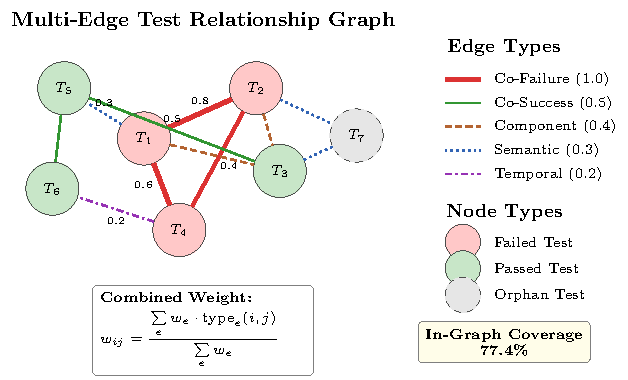
\includegraphics[width=\columnwidth]{figures/fig_multi_edge_graph.pdf}
    \caption{Test relationship graph with five edge types (illustrated for the
    industrial configuration). Co-failure edges (weight 1.0, solid) are the
    core graph used in all configurations and provide sufficient signal for
    effective prioritization (Section~\ref{sec:rq2}). Additional edge types
    (dashed) are optional extensions activated when richer metadata is
    available.}
    \label{fig:multiedge}
\end{figure}

\subsection{Core Architecture: Graph Attention Network}
\label{sec:fusion}

The core of \filopriori{} is a GATv2-based structural stream that processes
historical features over the test relationship graph. The architecture
additionally includes a semantic stream and cross-attention fusion module
as an \emph{exploratory investigation} into whether textual metadata
improves prioritization.

\textbf{Structural Stream (Graph Attention Network).}
The Structural Stream processes the 19 structural features
(Section~\ref{sec:feature_engineering}) over the test relationship graph
(Section~\ref{sec:graph}) using Graph Attention
Networks~\cite{velickovic2018graph}. The GAT architecture propagates
information between related test cases through the graph edges, allowing the
model to learn from the failure patterns of neighboring tests.

We use a single GATv2~\cite{brody2022attentive} layer with multi-head
attention. The layer computes:
\begin{equation}
    h_i' = \|_{k=1}^{H} \sigma\left(\sum_{j \in \mathcal{N}(i)} \alpha_{ij}^k \mathbf{W}^k h_j\right)
\end{equation}
where $H$ is the number of attention heads and $\alpha_{ij}^k$ are learned
attention coefficients for head $k$. In both evaluation settings, we use
$H = 2$ heads with a hidden dimension of 128, where each head produces a
128-dimensional output that is concatenated to yield a 256-dimensional
structural representation per test case (see Table~\ref{tab:arch_params}
for the complete configuration). The sensitivity analysis (Section~\ref{sec:rq4})
confirms that this shallow, 1-layer configuration with 2 heads outperforms
deeper architectures (2--3 layers) and more heads (4--8), suggesting that
test relationships can be effectively captured with a single message-passing
step.

The GAT layer incorporates the edge weights from the test relationship graph
(Section~\ref{sec:graph}) as initialization priors for the attention
computation. Crucially, GATv2's dynamic attention mechanism learns to
\emph{reweight} these priors during training: the attention coefficients
$\alpha_{ij}^k$ depend on both the query and key node features, so the model
can amplify or attenuate the fixed edge weights based on the actual predictive
value of each connection for each test case. This means the fixed weight
hierarchy (Table~\ref{tab:edge_types}) serves as a starting point, not a
rigid constraint.

\textbf{Exploratory: Semantic Stream and Cross-Attention Fusion.}
To investigate whether textual metadata improves prioritization beyond
structural features, we included a semantic stream that processes
Sentence-BERT embeddings (Section~\ref{sec:feature_engineering}) through a
feed-forward network with residual connections. The stream applies an input
projection layer (from the embedding dimension to 256) followed by two
residual feed-forward blocks~\cite{he2016deep}, each consisting of linear
expansion (256~$\rightarrow$~1,024), GELU activation, dropout (0.3), linear
compression (1,024~$\rightarrow$~256), dropout (0.3), and layer
normalization. The input dimensionality adapts to the available metadata
(1,536 when test and commit embeddings are concatenated; 768 when only test
names are available). The output is a 256-dimensional semantic
representation.

A Cross-Attention Fusion module combines semantic and structural
representations through bidirectional attention, allowing each modality to
attend to the other. This design choice enables the architecture to discover
correlations between textual content and behavioral patterns.

Specifically, the fusion operates in two directions. In the semantic-to-structural
direction, semantic features use the structural representations as context:
\begin{equation}
    h_{sem}' = h_{sem} + \text{MHA}(h_{sem}, h_{struct}, h_{struct})
\end{equation}
In the structural-to-semantic direction, structural features attend to the
semantic representations:
\begin{equation}
    h_{struct}' = h_{struct} + \text{MHA}(h_{struct}, h_{sem}, h_{sem})
\end{equation}
where $\text{MHA}(Q, K, V)$ denotes multi-head attention~\cite{vaswani2017attention}
with query $Q$, key $K$, and value $V$. Each attention operation uses 4 heads
with 256-dimensional queries, keys, and values, followed by layer normalization
for training stability. The residual connections in Equations~10 and~11 ensure
that the original representations are preserved while being enriched with
cross-modal information.

The attended features from both directions are then concatenated to form the
fused representation:
\begin{equation}
    h_{fused} = [h_{sem}' \| h_{struct}']
\end{equation}

The resulting 512-dimensional fused vector is passed to a classifier MLP
consisting of two hidden layers with dimensions [128, 64], each followed by
ReLU activation and dropout (0.4). The final output layer produces the
failure probability for each test case.

Figure~\ref{fig:architecture} illustrates the complete architecture
including the semantic stream and cross-attention fusion module.

\begin{figure}[!t]
    \centering
    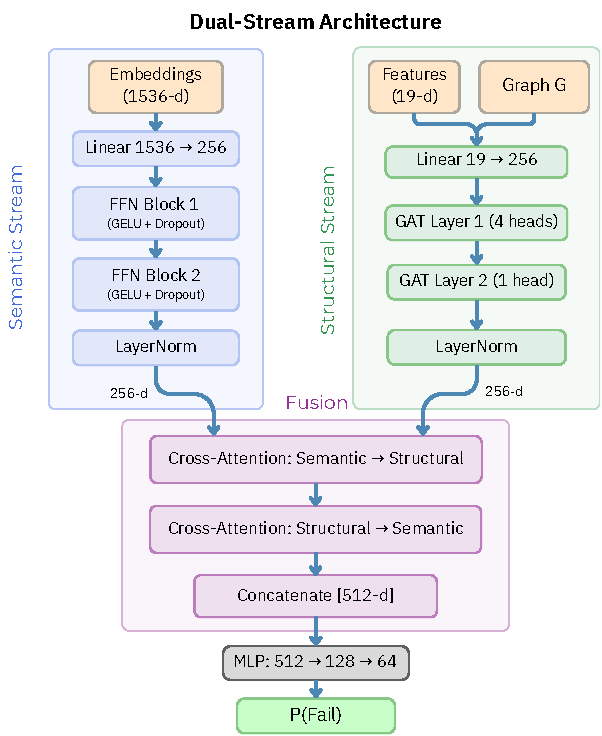
\includegraphics[width=0.9\columnwidth]{figures/fig_dual_stream_architecture_new.pdf}
    \caption{Architecture of \filopriori{}. The structural stream (left,
    solid border) is the core component, applying GATv2 over historical
    features using the co-failure test relationship graph. The semantic
    stream and cross-attention fusion (right, dashed border) were included
    as an exploratory investigation.}
    \label{fig:architecture}
\end{figure}

\subsection{Training Strategy}
\label{sec:training}

Test execution data typically exhibits severe class imbalance, with far more
passing tests than failing tests (e.g., 37:1 in our industrial dataset, and
up to 1,666:1 in some open-source projects). Addressing this imbalance
requires careful design, as multiple compensation mechanisms applied
simultaneously can cause over-correction. Through preliminary experiments,
we observed that combining class weights, balanced sampling, and focal $\alpha_f$
together led to mode collapse where the model predicted all samples as the
minority class.

Based on this empirical finding, we adopted a simplified dual-balancing
strategy that separates two complementary concerns: (1)~\emph{prior
correction} through balanced sampling, and (2)~\emph{gradient focusing}
through Focal Loss~\cite{lin2017focal} as the loss function:
\begin{equation}
    \mathcal{L} = -\alpha_f \cdot (1 - p_t)^\gamma \cdot \log(p_t)
\end{equation}
where the focal weighting parameter $\alpha_f = 0.75$ (mild minority bias)
and the focusing parameter $\gamma = 2.0$.
The $\alpha_f$ value is substantially lower than the prior triple-compensation
approach ($\alpha_f = 0.85$, Table~\ref{tab:balancing}), reducing the
class-weighting role of focal loss, while the $(1 - p_t)^\gamma$ modulating
factor with $\gamma = 2.0$ down-weights well-classified examples and
concentrates gradients on hard cases, providing a complementary signal to the
balanced sampler. The dual-balancing strategy outperformed the prior
triple-compensation approach on the validation set.

\textbf{Baseline Training Protocol.} Each deep learning baseline was evaluated
using its optimal class-imbalance mechanism as reported in its original
publication. DeepOrder employs a mathematically equivalent class prior weighting via \texttt{pos\_weight} in BCE
loss~\cite{chen2023deeporder}; NodeRank applies sklearn's algorithmic \texttt{class\_weight='balanced'}
option~\cite{li2024noderank}; TCP-Net relies on its original MSE regression formulation~\cite{abdelkarim2022tcp};
RETECS trains its reinforcement learning policy on unweighted samples~\cite{spieker2017reinforcement};
and FailRank-BB applies Logistic Regression with its optimal default configuration~\cite{hernandes2025method}.
We explicitly ensured that baselines received the same rigorous mitigation against class imbalance as
our method, whenever mathematically supported by their authors' designs, ensuring that performance
comparisons remain structurally fair and untampered.

\begin{table}[!t]
\centering
\caption{Simplified Dual-Balancing Configuration}
\label{tab:balancing}
\footnotesize
\begin{tabular}{lcc}
\toprule
\textbf{Mechanism} & \textbf{Triple-Comp.} & \textbf{Dual-Balancing} \\
\midrule
Class weights in loss & $19\times$ & \textbf{Disabled} \\
Focal $\alpha_f$ & $0.85$ ($1.7\times$) & $0.75$ (mild) \\
Balanced sampling & $20\times$ & $29\times$ (only) \\
\midrule
Effective weight & $\approx 646\times$ & $29\times$ \\
\bottomrule
\end{tabular}
\end{table}

The balanced sampler assigns minority weight 1.0 and majority weight 0.035
(ratio $\approx$29:1). This ratio was determined by grid search over values
ranging from 5:1 to 30:1 on the validation set, with 29:1 providing the best
trade-off between minority class recall and overall APFD. This strategy
ensures the minority class is adequately represented without over-compensation.
It is worth noting that this balancing strategy may need to be adjusted for
datasets with different class imbalance ratios. In datasets with moderate
imbalance, simpler approaches (e.g., standard cross-entropy) may suffice.

Both configurations use AdamW~\cite{loshchilov2019adamw} optimizer with
weight decay and early stopping, though the specific hyperparameters differ
to accommodate the different data scales: the industrial configuration uses a
lower learning rate ($3 \times 10^{-5}$) with cosine annealing and longer
training (80 epochs, patience 15), while the RTPTorrent configuration uses a
higher learning rate ($1 \times 10^{-3}$) with shorter training (30 epochs,
patience 7) per project. Table~\ref{tab:hyperparams} in
Section~\ref{sec:experimental} provides the complete training configuration
for each setting.

\textbf{Threshold Optimization.}
On the industrial dataset, we apply a two-phase threshold search on the
validation set to optimize the binary classification threshold for
$F_{\beta}$ ($\beta = 2.0$, favoring recall). Phase~1 scans [0.05, 0.90]
with step 0.05; Phase~2 refines around the best value with step 0.01.
The optimal threshold (0.28 vs.\ the default 0.50) substantially improves
minority class recall, contributing +1.0\% to APFD
(Table~\ref{tab:ablation}). This optimization is applied only on the
industrial dataset, where the continuous probability outputs benefit from
threshold calibration; on RTPTorrent, the ensemble scoring
(Section~\ref{sec:ensemble}) directly uses blended scores for ranking
without threshold conversion.

\subsection{Scoring Robustness Mechanisms}
\label{sec:deployment}

Beyond the core GATv2 classifier, \filopriori{} incorporates three
mechanisms that ensure robust scoring in practical deployment: (1)~a KNN
orphan scoring pipeline that handles test cases absent from the training
graph (Section~\ref{sec:orphan}); (2)~a DeepOrder-inspired DNN ensemble
with validation-optimized alpha blending that provides an independent
scoring channel (Section~\ref{sec:ensemble}); and (3)~automatic adaptation
logic that selects the active components based on the available metadata.

\textbf{Important scope note:} These mechanisms are activated selectively
depending on the deployment context
(Table~\ref{tab:rtptorrent_config}). In the metadata-rich configuration
(\textsc{Full}), the KNN orphan pipeline is the primary mechanism for
handling new test cases, and the GNN operates as the sole predictor. In
the metadata-sparse configuration (\textsc{Ensemble}), the DNN ensemble
inherently covers orphan tests through per-test temporal features
(requiring no graph membership), making the KNN pipeline unnecessary.
The remainder of this subsection details each mechanism with explicit
scope annotations.

\textbf{Orphan Test Problem.}
The GNN-based classifier produces accurate failure probabilities for test
cases present in the training graph. However, \emph{orphan tests} (test
cases that appear at inference time but were not present during
training) receive uniform scores from the GAT, effectively destroying
ranking capability for these tests. This is a fundamental limitation of any
graph-based approach: the GATv2 can only propagate information through nodes
it has seen during training. In CI environments, where new test cases are
frequently added, orphan handling is essential for practical deployment.

We address the orphan problem through two complementary mechanisms, each
suited to a different deployment context
(Table~\ref{tab:rtptorrent_config}):
\begin{itemize}
    \item \textbf{KNN-based node imputation}
    (\textsc{Filo-Priori-Full}): A four-stage pipeline that estimates
    orphan scores by finding the $k$ nearest in-graph neighbors via semantic
    and structural similarity, effectively imputing a virtual node
    embedding for the orphan test. This is applied when the GNN is the
    sole predictor (no DNN ensemble).
    \item \textbf{DNN ensemble coverage}
    (\textsc{Filo-Priori-Ensemble}): The DeepOrder-inspired DNN scores
    every test case based on per-test temporal features (failure rate,
    recency, etc.) \emph{without requiring graph membership}. Orphan tests
    are therefore automatically scored by the DNN component, and the
    $\alpha$-blending naturally incorporates these scores into the final
    ranking. When the DNN ensemble is active, explicit KNN imputation is
    unnecessary.
\end{itemize}

In our industrial dataset, 22.6\% of test cases in the evaluation set are
orphans, making this a significant practical concern. The two mechanisms
ensure that \filopriori{} handles orphan tests in both deployment contexts.

\textbf{KNN Orphan Scoring Pipeline} (\textsc{Full} configuration only).
\label{sec:orphan}

Figure~\ref{fig:orphan} illustrates the pipeline.

\textbf{Stage 1: KNN Similarity.} For each orphan test, we identify
$k=5$ nearest neighbors among in-graph tests using cosine similarity over
L2-normalized SBERT embeddings. This ensures that proximity reflects
semantic similarity rather than text length~\cite{reimers2019sentence}.

\textbf{Stage 2: Structural Blend.} We combine semantic similarity (from
embeddings) with structural similarity (from historical features) using a
blending weight $w_s = 0.35$:
\begin{equation}
    \text{sim}_{combined} = (1 - w_s) \cdot \text{sim}_{semantic} + w_s \cdot \text{sim}_{structural}
\end{equation}

\textbf{Stage 3: Temperature-Scaled Softmax.} We apply softmax with temperature
$T=0.7$ to concentrate weights on the most similar neighbors, reducing the
influence of dissimilar tests:
\begin{equation}
    w_i = \frac{\exp(\text{sim}_i / T)}{\sum_j \exp(\text{sim}_j / T)}
\end{equation}

\textbf{Stage 4: Orphan Blending.} The final orphan score blends the
KNN-weighted score with a base score (the GNN's default prediction for
unseen nodes) using a fixed blending weight:
\begin{equation}
    \text{score}_{orphan} = \alpha_o \cdot \sum_i w_i \cdot \text{score}_i + (1-\alpha_o) \cdot \text{score}_{base}
\end{equation}
where $\alpha_o = 0.55$ is tuned on the validation set. This balances the
signal from similar in-graph neighbors against the GNN's prior, preventing
over-reliance on the KNN estimate when the neighborhood is sparse or
dissimilar.

The hyperparameters of this pipeline ($k=5$, $w_s=0.35$, $T=0.7$) were tuned on the validation set.
Before orphan handling, orphan scores had zero variance (all 0.50). After
applying the pipeline, scores range from 0.29 to 0.51 with std=0.046,
enabling effective ranking among orphan tests.

\begin{figure}[!t]
    \centering
    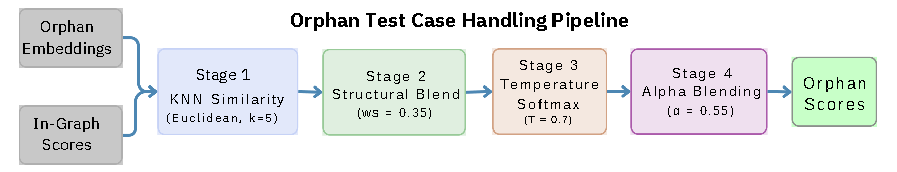
\includegraphics[width=\columnwidth]{figures/fig_orphan_pipeline_new.pdf}
    \caption{Four-stage orphan handling pipeline. Orphan test cases are scored using
    KNN similarity to in-graph tests, with structural blending and temperature-scaled
    softmax to concentrate weights on the most similar neighbors.}
    \label{fig:orphan}
\end{figure}

\textbf{DNN Ensemble with Alpha Blending} (active in both configurations;
primary scoring channel in \textsc{Ensemble}).
\label{sec:ensemble}

The two predictors are combined
through validation-optimized alpha blending, allowing the framework to
automatically favor the stronger predictor for each deployment context.
The DNN ensemble comprises three tightly coupled components described
below: the DNN architecture itself, a history pre-warming strategy, and
a validation-optimized alpha blending mechanism.

\emph{DNN Architecture.}
We train a separate feedforward neural network with three hidden layers
(64, 32, 16 neurons) and sigmoid output activation, taking as input 8
historical features per test case: the last execution result, failure
proportions in the last 1, 2, 3, 5, and 10 executions, normalized cycles
since last failure, and total status changes. The DNN is trained per
project using Binary Cross-Entropy (BCE) loss with manual class weighting:
\begin{equation}
    \mathcal{L}_{DNN} = -\frac{1}{N}\sum_{i=1}^{N} w_i \cdot \bigl[
    y_i \log(\hat{y}_i) + (1{-}y_i)\log(1{-}\hat{y}_i) \bigr]
\end{equation}
where $w_i = w_{pos}$ if $y_i = 1$ (failure) and $w_i = 1$ otherwise.
The positive class weight $w_{pos}$ is computed as the ratio of passing to
failing tests in the training set, \emph{clamped} to a maximum of 50 to
prevent training instability in projects with very rare failures (e.g., a
project with 0.06\% failure rate would yield $w_{pos} \approx 1{,}666$
without clamping, causing the DNN to predict all tests as failures).

\emph{History Pre-Warming.}
To provide the DNN with complete historical context, we process \emph{all}
training builds chronologically to accumulate execution history features
(a fast $O(n)$ operation that only updates running counters), then train
the DNN on only the last 5,000 builds with full history context. This
ensures that features such as ``failure rate in the last 10 executions''
reflect the complete available history rather than being computed from a
truncated window. Importantly, all history-based baselines (DeepOrder,
TCP-Net) receive the same training data: the complete set of
temporally-ordered training builds. The pre-warming step does not provide
\filopriori{} with additional data beyond what baselines receive; it merely
separates the history accumulation phase from the DNN weight optimization
phase for computational efficiency on large projects.

\emph{Alpha Blending.}
The final prioritization score for each test case combines both predictors
through a linear blend:
\begin{equation}
    \text{score}_{final} = \alpha \cdot P_{GNN}(\text{fail}) +
    (1 - \alpha) \cdot S_{DNN}
\end{equation}
where $P_{GNN}(\text{fail})$ is the failure probability from the
dual-stream GATv2 model and $S_{DNN}$ is the DNN output score. The
blending coefficient $\alpha \in \{0.0, 0.1, \ldots, 0.9\}$ is selected
per project by maximizing APFD on a held-out validation set (10\% of
training builds, temporally ordered). The range excludes $\alpha = 1.0$
(pure GNN) to ensure the DNN always retains nonzero weight as a safety
mechanism for orphan test coverage; the DNN ensemble verification on the
industrial dataset (Section~\ref{sec:rq2}) separately evaluates
$\alpha = 1.0$ and confirms it is optimal when graph density is high.
To guard against unreliable alpha selection in projects with few failures,
we require at least 3 validation builds containing failures; projects
below this threshold default to $\alpha = 0.5$.

This ensemble approach is motivated by the complementary strengths of
the two predictors: the GNN captures inter-test structural relationships
through graph message passing, while the DNN captures per-test temporal
failure dynamics independently. On the RTPTorrent benchmark, the optimal
$\alpha$ varies substantially across projects (from 0.0 to 0.9),
confirming that the relative value of each predictor is
project-dependent.

\textbf{Automatic Adaptation.}
In deployment, adaptation occurs automatically through two data-driven
mechanisms rather than manual component selection. First, the graph
construction uses only the edge types supported
by the available metadata: absent metadata simply produces no edges,
naturally reducing the graph to co-failure edges without intervention.
Second, the alpha blending coefficient is optimized on the validation set:
when the GNN is strong (rich metadata), the optimizer selects
$\alpha \approx 1.0$; when the DNN is stronger (sparse metadata), it
selects $\alpha \approx 0.0$. The DNN also inherently scores orphan tests
without requiring graph membership, complementing the KNN pipeline. In
practice, the only human decision is which textual fields to encode; the
rest adapts automatically. Table~\ref{tab:rtptorrent_config} summarizes
the two configurations evaluated in this work.

%------------------------------------------------------------------------------
% SECTION 5: EXPERIMENTAL DESIGN
%------------------------------------------------------------------------------
\section{Experimental Design}
\label{sec:experimental}

All hyperparameters, classification thresholds, and edge weights reported
in this paper were selected exclusively on temporally held-out validation
data, never on the test partition. On the industrial dataset, grid search
was conducted on the validation split (chronologically preceding the test
builds); on RTPTorrent, per-project validation sets (10\% of training
builds, temporally ordered) were used for alpha blending optimization and
early stopping. This strict temporal separation between tuning and
evaluation prevents data leakage and ensures that the reported APFD
values reflect genuine predictive performance on unseen future builds.

\subsection{Research Questions}

The experiments are designed to answer four research questions that assess
\filopriori{} from complementary perspectives:

\begin{itemize}
    \item \textbf{RQ1 (Effectiveness)}: Can modeling structural relationships
    between test cases through graph neural networks improve fault detection
    compared to approaches that treat tests independently? This question evaluates
    the overall TCP performance on two datasets, comparing against both heuristic
    and learning-based baselines.
    \item \textbf{RQ2 (Components)}: Which architectural components contribute
    most to the effectiveness of graph-based test case prioritization? This question
    isolates the impact of each innovation through an ablation study on the
    industrial dataset.
    \item \textbf{RQ3 (Robustness)}: How robust is the proposed approach when
    applied to builds from different time periods than those used for training?
    This question assesses temporal generalization by training on earlier builds
    and testing on later ones.
    \item \textbf{RQ4 (Sensitivity)}: How sensitive is the approach to the choice
    of key hyperparameters? This question analyzes the impact of key configuration
    parameters on performance.
\end{itemize}

\subsection{Datasets}

We evaluate \filopriori{} on two complementary datasets spanning industrial
software testing and open-source CI environments.

\textbf{Dataset 1: Industrial QTA Dataset.} The QTA (Qodo Test Automation) dataset
comes from a commercial mobile device CI pipeline. The data is organized by
\emph{builds}, where each build represents a complete cycle of code integration and
testing triggered by code changes. Each build contains multiple test case
executions, and the same test case may appear across different builds with
different outcomes. This dataset provides rich semantic information:
test case summaries and detailed steps (forming the semantic component) as well as
commit messages and code diffs associated with each build. The structural component
is derived from the historical execution records, which include the outcome
(pass/fail) of each test case in each build, timestamps, and associated change
requests. Table~\ref{tab:dataset_qta} summarizes its statistics.

The anonymized version provided in the replication package preserves the
properties essential for reproduction: (1)~temporal ordering of builds is
maintained (build timestamps are replaced with monotonically increasing
indices); (2)~test case identities are replaced with opaque identifiers while
preserving the pass/fail outcome sequence and co-occurrence patterns;
(3)~semantic text (test descriptions, commit messages) is replaced with
Sentence-BERT embedding vectors, preserving the semantic similarity structure
without exposing proprietary content; and (4)~all structural features
(failure rate, recency, execution time) are computed from the anonymized
records and included directly.

\begin{table}[!t]
\centering
\caption{Industrial QTA Dataset Statistics}
\label{tab:dataset_qta}
\begin{tabular}{lr}
\toprule
\textbf{Statistic} & \textbf{Value} \\
\midrule
Total test executions & 52,102 \\
Unique builds & 1,339 \\
Builds with failures & 277 (20.7\%) \\
Unique test cases & 2,347 \\
Pass:Fail ratio & 37:1 \\
Semantic info & Rich (descriptions, steps, commits) \\
Structural info & Execution history, failure patterns \\
\bottomrule
\end{tabular}
\end{table}

\textbf{Dataset 2: RTPTorrent Open-Source Dataset.} To evaluate generalization
across diverse open-source projects, we use the RTPTorrent
dataset~\cite{mattis2020rtptorrent}, an open-source benchmark from MSR 2020
containing test execution histories from 20 Java projects on GitHub with over
100,000 Travis CI build logs. Unlike the industrial dataset, RTPTorrent does not
contain commit messages or detailed test descriptions; the semantic component is
limited to test class and method names. The structural component is derived from
the execution history available in the CI build logs, including pass/fail
outcomes and execution timestamps. For this dataset, we deploy the
\textbf{ensemble variant} described in Section~\ref{sec:ensemble}, which
differs from the full industrial pipeline in the following ways:
(1)~the semantic stream processes only test class/method names (no
descriptions, steps, or commit messages); (2)~the graph uses only
co-failure edges (component and temporal metadata are unavailable);
(3)~a DeepOrder-inspired DNN is trained independently per project and
combined with the GATv2 model through validation-optimized alpha blending;
and (4)~orphan test cases are handled by the DNN ensemble component, which
scores all tests through per-test historical features regardless of graph
membership (Section~\ref{sec:deployment}), making the KNN node imputation
pipeline unnecessary.
Table~\ref{tab:rtptorrent_config} summarizes the key configuration
differences between the two evaluation settings, and
Table~\ref{tab:dataset_rtptorrent} summarizes the dataset statistics.

\begin{table}[!t]
\centering
\caption{Adaptive Pipeline Configurations: Components Activated by Metadata Availability}
\label{tab:rtptorrent_config}
\footnotesize
\begin{tabular}{lcc}
\toprule
\textbf{Aspect} & \textbf{\textsc{Full}} & \textbf{\textsc{Ensemble}} \\
 & \textbf{(Industrial)} & \textbf{(RTPTorrent)} \\
\midrule
Core model & GATv2 & GATv2 + DNN \\
Graph edges & 5 types & Co-failure only \\
Semantic input & Rich (desc., commits) & Test names only \\
Orphan handling & KNN node imputation & DNN ensemble \\
Learning rate & $3{\times}10^{-5}$ & $1{\times}10^{-3}$ \\
Score & GNN probability & $\alpha$-blending \\
\bottomrule
\end{tabular}
\end{table}

\begin{table}[!t]
\centering
\caption{RTPTorrent Dataset Statistics}
\label{tab:dataset_rtptorrent}
\begin{tabular}{lr}
\toprule
\textbf{Statistic} & \textbf{Value} \\
\midrule
Projects & 20 Java projects \\
Total builds & $>$100,000 \\
Source & Travis CI build logs \\
Semantic info & Limited (test names only) \\
Structural info & Execution history, timestamps \\
License & CC BY 4.0 \\
\bottomrule
\end{tabular}
\end{table}

The complementary nature of these two datasets enables comprehensive evaluation:
the industrial dataset tests the full \filopriori{} pipeline with rich semantic
features (test descriptions, commit messages, and code diffs), while RTPTorrent
tests cross-project generalization in open-source environments with limited
semantic information (test names only). Together, they cover both extremes of
the semantic information spectrum and span controlled industrial settings and
diverse open-source projects.

\subsection{Baselines}

We compare \filopriori{} against baselines from two categories, following common
practice in TCP evaluation~\cite{elbaum2002test, chen2023deeporder}.

\textbf{Heuristic Baselines} represent simple, interpretable strategies commonly
used in practice and in TCP research as reference points:
\begin{itemize}
    \item \textbf{Random}: Random ordering of test cases, providing the expected
    baseline of APFD $\approx$ 0.5. This serves as the lower bound for any
    meaningful prioritization strategy.
    \item \textbf{Recency}: Prioritizes tests that failed most recently, based on
    Kim and Porter's~\cite{kim2002history} finding that recently failed tests are
    more likely to fail again.
    \item \textbf{RecentFailureRate}: Ranks tests by their failure rate in the
    last 5 builds, capturing short-term failure trends.
    \item \textbf{FailureRate}: Ranks tests by their overall historical failure
    rate, providing a long-term perspective.
    \item \textbf{GreedyHistorical}: At each step, selects the highest-scoring
    unranked test case according to a composite priority function that
    combines three signals: (1)~recency of last failure (tests that failed
    more recently receive higher priority), (2)~historical failure rate
    (tests with higher cumulative failure ratios are preferred), and
    (3)~test age (newer tests are prioritized over older, well-exercised
    ones). The selection is greedy in the sense that it ranks tests one at
    a time without backtracking. Once a test is placed at position $k$, it
    is never reconsidered.
\end{itemize}

We compare against five state-of-the-art deep learning approaches:
\begin{itemize}
    \item \textbf{DeepOrder}~\cite{chen2023deeporder}: A deep neural network
    that uses 8 historical features per test case (including last execution
    result, time since last failure, and failure rate) to predict failure
    likelihood. DeepOrder treats test cases independently without modeling
    relationships between them.
    \item \textbf{TCP-Net}~\cite{abdelkarim2022tcp}: An end-to-end deep neural
    network that learns directly from historical execution features and temporal
    patterns to predict test failure probability for ranking.
    \item \textbf{NodeRank}~\cite{li2024noderank}: A mutation-based analysis
    approach that uses ensemble learning (LightGBM and Random Forest) with
    graph structure, node feature, and model weight mutations to compute
    priority scores. Originally designed for GNN model testing, we adapt it
    to software TCP by applying mutations to the test relationship graph and
    structural features (see Section~\ref{sec:related}).
    \item \textbf{RETECS}~\cite{spieker2017reinforcement}: A reinforcement
    learning approach that frames TCP as a sequential decision problem, learning
    to prioritize tests by maximizing a reward signal based on fault detection
    across CI cycles.
    \item \textbf{FailRank-BB}~\cite{hernandes2025method}: A semantic-based
    approach that uses Sentence-BERT embeddings of test case descriptions and
    commit messages with Logistic Regression for binary classification.
    FailRank-BB leverages rich textual information but does not model structural
    relationships between test cases or employ graph-based architectures.
\end{itemize}

\subsection{Evaluation Metrics}

We use APFD (Average Percentage of Faults Detected) as the primary evaluation
metric, computed per build and averaged across all builds containing at least
one failure. APFD measures how early in the test execution sequence faults are
detected, with higher values indicating better prioritization (see
Section~\ref{sec:bg_apfd} for the formal definition).

For statistical comparison between \filopriori{} and each baseline, we use the
Wilcoxon signed-rank test~\cite{wilcoxon1945individual} with significance level
$\alpha = 0.05$. On the industrial dataset, the test is computed on paired
per-build APFD values ($n = 277$ builds with failures). On RTPTorrent, the
test is computed on paired per-project mean APFD values ($n = 20$ projects),
which avoids intra-project autocorrelation but limits statistical power.
Following the guidelines of Arcuri and Briand~\cite{arcuri2011practical},
we report Cliff's delta ($\delta$) as a non-parametric effect size measure
alongside p-values. We use the thresholds of Romano et al.:
$|\delta| < 0.147$ (negligible), $< 0.33$ (small), $< 0.474$ (medium),
$\geq 0.474$ (large). We also report percentage improvement ($\Delta$)
for practical interpretation.

\subsection{Implementation Details}

All experiments use PyTorch 2.0 with PyTorch Geometric 2.3 on an NVIDIA RTX
3090 (24GB VRAM).

\textbf{Baseline provenance.} All five baselines were reimplemented
following their published descriptions and validated on publicly available
data where possible. DeepOrder~\cite{chen2023deeporder} and
RETECS~\cite{spieker2017reinforcement} were reimplemented from their
published algorithms. TCP-Net~\cite{abdelkarim2022tcp} and
FailRank-BB~\cite{hernandes2025method} were reimplemented following their
respective papers. NodeRank~\cite{li2024noderank} was adapted from its
original GNN testing domain to TCP (see Section~\ref{sec:related}).
All baseline implementations are included in the replication package for
independent verification.

Table~\ref{tab:hyperparams} lists the training
hyperparameters for each evaluation setting. On the industrial dataset, the
GNN is trained with AdamW using cosine annealing and early stopping. On
RTPTorrent, the GNN and the DeepOrder DNN are trained independently per
project: the DNN uses the last 5,000 builds (with full history pre-warmed
from all prior builds) and its own optimizer, while the GNN uses the same
AdamW configuration with a higher learning rate suited to the per-project
training regime.

\begin{table}[!t]
\centering
\caption{Training Hyperparameters by Evaluation Setting}
\label{tab:hyperparams}
\footnotesize
\begin{tabular}{lccc}
\toprule
 & \textbf{Industrial} & \multicolumn{2}{c}{\textbf{RTPTorrent}} \\
\cmidrule(lr){3-4}
\textbf{Hyperparameter} & \textbf{(GNN)} & \textbf{GNN} & \textbf{DNN} \\
\midrule
Optimizer & AdamW & AdamW & Adam \\
Learning rate & $3 \times 10^{-5}$ & $1 \times 10^{-3}$ & $1 \times 10^{-3}$ \\
Weight decay & $1 \times 10^{-4}$ & $1 \times 10^{-4}$ & -- \\
Batch size & 16 & per-build & 128 \\
Max epochs & 80 & 30 & 15 \\
Early stopping & patience 15 & patience 7 & -- \\
Scheduler & cosine & -- & -- \\
Gradient clip & 1.0 & -- & -- \\
\bottomrule
\end{tabular}
\end{table}

\begin{table}[!t]
\centering
\caption{Model Architecture and Pipeline Parameters}
\label{tab:arch_params}
\footnotesize
\begin{tabular}{lcc}
\toprule
\textbf{Parameter} & \textbf{Industrial} & \textbf{RTPTorrent} \\
\midrule
\multicolumn{3}{l}{\textit{GNN Architecture}} \\
GAT layers & 1 & 1 \\
Attention heads & 2 & 2 \\
GAT hidden dim & 128 & 128 \\
Structural input dim & 19 & 19 \\
Semantic input dim & 1536 & 768 \\
Semantic hidden dim & 256 & 256 \\
Structural hidden dim & 64 & 64 \\
\midrule
\multicolumn{3}{l}{\textit{Graph Construction}} \\
Edge types & 5 & co-failure only \\
Semantic threshold & 0.65 & -- \\
Max neighbors & 10 & -- \\
\midrule
\multicolumn{3}{l}{\textit{Class Balancing}} \\
Balanced sampling ratio & 29:1 & -- \\
Focal $\alpha_f$ / $\gamma$ & 0.75 / 2.0 & -- / 2.0 \\
DNN pos\_weight (max) & -- & 50.0 \\
\midrule
\multicolumn{3}{l}{\textit{Pipeline}} \\
Orphan KNN ($k$, $\alpha_o$, $T$) & 5, 0.55, 0.7 & not applied \\
DNN hidden layers & -- & 64, 32, 16 \\
Alpha blending range & -- & $[0.0, 0.1, \ldots, 0.9]$ \\
Max training builds (DNN) & -- & 5,000 \\
\bottomrule
\end{tabular}
\end{table}

%------------------------------------------------------------------------------
% SECTION 6: RESULTS
%------------------------------------------------------------------------------
\section{Results}
\label{sec:results}

%%%%%%%%%%%%%%%%%%%%%%%%%%%%%%%%%%%%%%%%%%%%%%%%%%%%%%%%%%%%%%%%%%%%%%%%%%%%%%%
% SECTION: RESULTS (IEEE TSE Format) — Updated with Consolidated Results
%%%%%%%%%%%%%%%%%%%%%%%%%%%%%%%%%%%%%%%%%%%%%%%%%%%%%%%%%%%%%%%%%%%%%%%%%%%%%%%

% Note: Section header is in main_ieee_tse.tex

This section presents the experimental results organized by research questions.
The experiments address the four research questions defined in
Section~\ref{sec:experimental}, evaluating \filopriori{} across two
complementary datasets against five state-of-the-art deep learning baselines.

%------------------------------------------------------------------------------
% RQ1: Effectiveness on Industrial Dataset
%------------------------------------------------------------------------------

\subsection{RQ1: Effectiveness on Industrial Dataset}
\label{sec:rq1}

Table~\ref{tab:tcp_comparison} presents the comparison of \filopriori{} against
five deep learning baselines on the industrial QTA dataset (277 builds with at
least one failure). We use APFD as the primary metric with Wilcoxon signed-rank
tests for statistical significance.

\begin{table}[!t]
\centering
\caption{Comparison with Deep Learning Baselines (Industrial Dataset, 277 Builds)}
\label{tab:tcp_comparison}
\scriptsize
\begin{tabular}{lccccr}
\toprule
\textbf{Method} & \textbf{APFD} & \textbf{Std} & \textbf{p} & \textbf{$\delta$} & \textbf{$\Delta$} \\
\midrule
\textbf{\filopriori{}} & \textbf{0.761} & \textbf{0.189} & -- & -- & -- \\
DeepOrder~\cite{chen2023deeporder} & 0.689 & 0.266 & $<$0.001 & 0.10 (N) & +10.2\% \\
TCP-Net~\cite{abdelkarim2022tcp} & 0.670 & 0.271 & $<$0.001 & 0.14 (N) & +13.3\% \\
NodeRank~\cite{li2024noderank} & 0.661 & 0.270 & $<$0.001 & 0.14 (N) & +14.9\% \\
RETECS~\cite{spieker2017reinforcement} & 0.641 & 0.281 & $<$0.001 & 0.21 (S) & +18.6\% \\
FailRank-BB~\cite{hernandes2025method} & 0.595 & 0.263 & $<$0.001 & 0.35 (M) & +27.6\% \\
\bottomrule
\end{tabular}
\begin{tablenotes}
\small
\item *** $p < 0.001$ (Wilcoxon signed-rank test vs \filopriori{}).
\item $\delta$: Cliff's delta effect size. N = negligible ($<$0.147), S = small ($<$0.33),
M = medium ($<$0.474), L = large ($\geq$0.474)~\cite{arcuri2011practical}.
\item All methods evaluated on the same 277 builds with at least one failure.
\end{tablenotes}
\end{table}

\filopriori{} achieves a mean APFD of \textbf{0.7611} (std: 0.189),
outperforming all five deep learning baselines with statistical significance
($p < 0.001$). The improvements range from +10.2\% over DeepOrder (the
strongest baseline) to +27.6\% over FailRank-BB (the weakest).
Cliff's delta effect sizes range from negligible ($\delta = 0.10$, DeepOrder)
to medium ($\delta = 0.35$, FailRank-BB). The apparent discrepancy between
the large percentage improvements (+10.2\% to +27.6\% in mean APFD) and the
small-to-negligible per-build effect sizes reflects a fundamental difference
between the two measures: the percentage improvement captures the aggregate
shift in mean APFD across all 277 builds, while Cliff's delta measures how
often one method dominates the other on individual builds. A negligible
$\delta$ (e.g., 0.10 vs.\ DeepOrder) means that \filopriori{} outperforms
DeepOrder on only slightly more than half of the builds, but when it does
outperform, the APFD gains are substantially larger than the losses on the
builds where it underperforms, producing a meaningful shift in the mean.
This pattern is characteristic of TCP tasks with heavy-tailed build
distributions: a minority of builds with concentrated failures benefit
disproportionately from graph-based modeling, while simpler builds (with
few tests or obvious failure patterns) show little difference between methods.
The practical implication is that \filopriori{}'s advantage is concentrated on
the builds where prioritization matters most, specifically those with complex, non-trivial
failure patterns.

These results suggest that \filopriori{}'s multi-edge graph architecture effectively
exploits the rich structural information available in the
industrial dataset, even under strict temporal validation. DeepOrder and TCP-Net rely solely on historical features
without modeling relationships between test cases. RETECS, as a reinforcement
learning approach, struggles with the extreme sparsity of the reward signal inherent
in the 37:1 class imbalance, failing to optimize its ranking policy effectively. NodeRank,
while graph-based, relies on mutation sensitivity heuristics that are less effective at
isolating discriminative failure patterns than explicit message passing. FailRank-BB leverages semantic embeddings but relies on
Logistic Regression without graph-based modeling, which appears insufficient for
capturing the complex dependencies present in industrial test suites.

\textbf{Comparison with Heuristic Baselines.}
Table~\ref{tab:heuristic_industry} compares \filopriori{} against five
heuristic baselines on the industrial dataset. The strongest heuristic,
FailureRate (APFD = 0.664), outperforms Random (0.537) by a substantial
margin, confirming that historical failure patterns carry significant
predictive signal. However, \filopriori{} outperforms all heuristics by
at least +14.6\%, and the strongest deep learning baseline
(DeepOrder, APFD = 0.689) also exceeds all heuristics, validating our
choice to focus the main comparison on deep learning methods. Notably,
Recency (APFD = 0.420) performs \emph{below} random ordering on this
dataset. This contrasts with its strong performance on RTPTorrent
(Table~\ref{tab:rtptorrent_heuristic}), where recently\_failed achieves
0.821. The disparity is explained by the industrial test suite's
characteristics: with a 37:1 Pass:Fail ratio and long intervals between
failures for most tests, simple recency is a poor predictor; the more
informative signal comes from cumulative failure rates, which both
FailureRate and the deep learning baselines capture.

\begin{table}[!t]
\centering
\caption{Heuristic Baseline Comparison (Industrial Dataset, 277 Builds)}
\label{tab:heuristic_industry}
\scriptsize
\begin{tabular}{lccr}
\toprule
\textbf{Baseline} & \textbf{APFD} & \textbf{Std} & \textbf{$\Delta$ vs \filopriori{}} \\
\midrule
\textbf{\filopriori{}} & \textbf{0.761} & \textbf{0.189} & -- \\
FailureRate & 0.664 & 0.269 & +14.6\% \\
RecentFailureRate & 0.658 & 0.269 & +15.7\% \\
GreedyHistorical & 0.657 & 0.274 & +15.8\% \\
Random & 0.537 & 0.272 & +41.7\% \\
Recency & 0.420 & 0.313 & +81.2\% \\
\bottomrule
\end{tabular}
\begin{tablenotes}
\small
\item All heuristics use temporally accumulated history (no future leakage).
\item Recency ranks tests by builds since last failure. FailureRate
ranks by overall historical failure rate.
\end{tablenotes}
\end{table}

\textbf{Isolating Architectural vs.\ Balancing Contributions.}
A potential confound in the baseline comparison is that \filopriori{} uses a
different class-imbalance strategy (dual-balancing: balanced sampling at 29:1
+ focal loss) than the baselines, which use their native strategies. To
isolate whether \filopriori{}'s advantage stems from the GATv2 graph
architecture or from the balancing strategy, we retrained DeepOrder (the
strongest baseline, APFD = 0.689) using \filopriori{}'s dual-balancing
protocol, keeping all other aspects of DeepOrder unchanged (same 8 features,
same network architecture, same evaluation).
Table~\ref{tab:deeporder_dualbalancing} presents the results.

\begin{table}[!t]
\centering
\caption{Isolating Architectural vs.\ Balancing Contributions (Industrial
Dataset). DeepOrder retrained with \filopriori{}'s dual-balancing strategy.}
\label{tab:deeporder_dualbalancing}
\footnotesize
\begin{tabular}{lcc}
\toprule
\textbf{Configuration} & \textbf{APFD} & \textbf{$\Delta$ vs \filopriori{}} \\
\midrule
\filopriori{} (Full) & 0.761 & -- \\
\filopriori{} w/o Dual-Balancing & 0.729 & $-$4.0\% \\
\midrule
DeepOrder (original BCE) & 0.689 & $-$9.4\% \\
DeepOrder + Balanced Sampling & 0.687 & $-$9.7\% \\
DeepOrder + Dual-Balancing & 0.676 & $-$11.3\% \\
\bottomrule
\end{tabular}
\begin{tablenotes}
\small
\item Dual-Balancing = Balanced Sampling (29:1) + Focal Loss ($\alpha_f\!=\!0.75$, $\gamma\!=\!2.0$).
\item All configurations use the same 277 test builds and identical evaluation protocol.
\end{tablenotes}
\end{table}

DeepOrder with \filopriori{}'s dual-balancing achieves APFD = 0.676,
\emph{below} its original score (0.689, $-$1.9\%), and 11.3\% below
\filopriori{} (0.761). The balanced-sampling-only variant (0.687) is also
marginally below the original. This demonstrates that \filopriori{}'s
balancing strategy is not transferable to DeepOrder's architecture:
the dual-balancing was co-optimized with the GATv2 architecture, and
applying it to a flat-feature DNN slightly disrupts its native training
dynamics. Crucially, the 9.7\% gap between the best DeepOrder variant
(0.687) and \filopriori{} (0.761) is primarily attributable to the GATv2
graph architecture, confirming that the graph-based structural modeling
provides genuine advantages beyond class-imbalance handling.

%------------------------------------------------------------------------------
% RQ1: Effectiveness on RTPTorrent
%------------------------------------------------------------------------------

\subsection{RQ1: Effectiveness on RTPTorrent}
\label{sec:rq1_rtptorrent}

To evaluate generalization across diverse open-source projects, we
conducted experiments on the RTPTorrent benchmark~\cite{mattis2020rtptorrent},
which contains test execution histories from 20 Java projects with over 100,000
Travis CI builds. We evaluated \filopriori{} using its ensemble architecture
(Section~\ref{sec:ensemble}), trained independently on each project.

\textbf{Comparison with Deep Learning Baselines.}
Table~\ref{tab:rtptorrent_dl} presents the aggregate results of \filopriori{}
against the five deep learning baselines on the RTPTorrent dataset.

\begin{table}[!t]
\centering
\caption{Deep Learning Baseline Comparison (RTPTorrent, 20 Projects)}
\label{tab:rtptorrent_dl}
\scriptsize
\begin{tabular}{lcccccr}
\toprule
\textbf{Method} & \textbf{APFD} & \textbf{Std} & \textbf{N} & \textbf{p} & \textbf{$\delta$} & \textbf{$\Delta$} \\
\midrule
\textbf{\filopriori{}} & \textbf{0.854} & \textbf{0.111} & 2,937 & -- & -- & -- \\
TCP-Net~\cite{abdelkarim2022tcp} & 0.825 & 0.110 & 2,937 & 0.087 & 0.08 (N) & +1.6\% \\
FailRank-BB~\cite{hernandes2025method} & 0.822 & 0.092 & 2,937 & 0.046* & 0.15 (S) & +2.0\% \\
DeepOrder~\cite{chen2023deeporder} & 0.814 & 0.104 & 2,937 & 0.018* & 0.16 (S) & +3.0\% \\
NodeRank~\cite{li2024noderank} & 0.809 & 0.114 & 2,937 & 0.009** & 0.20 (S) & +5.6\% \\
RETECS~\cite{spieker2017reinforcement} & 0.679 & 0.156 & 2,937 & $<$0.001 & 0.65 (L) & +23.5\% \\
\bottomrule
\end{tabular}
\begin{tablenotes}
\small
\item Grand mean APFD computed as the average of 20 per-project mean APFD values.
\item Wilcoxon signed-rank tests and Cliff's $\delta$ computed on the 20 paired per-project means ($n = 20$).
\item $\delta$: Cliff's delta. N = negligible, S = small, M = medium, L = large~\cite{arcuri2011practical}.
\item All methods evaluated on the same 2,937 builds with failures across 20 projects.
\end{tablenotes}
\end{table}

\filopriori{} achieves the highest aggregate APFD (0.8540) among all
evaluated methods, with statistically significant improvements over four of
five deep learning baselines: FailRank-BB (+2.0\%, $p=0.046$), DeepOrder
(+3.0\%, $p=0.018$), NodeRank (+5.6\%, $p=0.009$), and RETECS (+23.5\%,
$p<0.001$). The difference from TCP-Net (+1.6\%, $p=0.087$) does not reach
statistical significance at $\alpha=0.05$.

\textbf{Multiple-comparison correction.} Applying Holm-Bonferroni correction
to the five pairwise comparisons renders the differences from TCP-Net
($p=0.087$, not significant before correction) and FailRank-BB ($p=0.046$,
adjusted $\approx 0.18$) non-significant. DeepOrder ($p=0.018$, adjusted
$\approx 0.054$) is marginal. Only NodeRank ($p=0.009$) and RETECS
($p<0.001$) remain significant after correction. The RTPTorrent results
show that \filopriori{} achieves the numerically highest APFD with
statistically robust improvements over NodeRank and RETECS, while the
differences from TCP-Net, FailRank-BB, and DeepOrder should be interpreted
with caution.

Cliff's delta effect sizes on the 20 paired per-project means confirm
these patterns: the effect vs.\ RETECS is large ($\delta = 0.65$),
vs.\ NodeRank and DeepOrder small ($\delta = 0.20$ and $0.16$),
and vs.\ TCP-Net negligible ($\delta = 0.08$) and vs.\ FailRank-BB small ($\delta = 0.15$).
These small-to-negligible effect sizes for the top baselines,
combined with the limited statistical power ($n = 20$ paired observations),
are consistent with the multiple-comparison analysis above.
The reduced margin relative to the industrial dataset is consistent with the
limited semantic information available in RTPTorrent (test names only, no
descriptions or commits), which constrains the advantage of \filopriori{}'s
semantic stream.

\textbf{Comparison with Heuristic Baselines.}
Table~\ref{tab:rtptorrent_heuristic} compares \filopriori{} against the
standard heuristic baselines provided with the RTPTorrent benchmark.

\begin{table}[!t]
\centering
\caption{Heuristic Baseline Comparison (RTPTorrent, 20 Projects)}
\label{tab:rtptorrent_heuristic}
\scriptsize
\begin{tabular}{lccr}
\toprule
\textbf{Baseline} & \textbf{APFD} & \textbf{$\Delta$ vs \filopriori{}} & \textbf{p-value} \\
\midrule
optimal\_failure (oracle) & 0.9249 & -9.3\% & -- \\
\textbf{\filopriori{}} & \textbf{0.8540} & -- & -- \\
recently\_failed & 0.8209 & +2.1\% & sig.* \\
optimal\_duration & 0.5934 & +41.3\% & $<$0.001*** \\
matrix\_naive & 0.5693 & +47.3\% & $<$0.001*** \\
random & 0.4940 & +69.7\% & $<$0.001*** \\
matrix\_conditional & 0.5132 & +63.4\% & $<$0.001*** \\
untreated & 0.3574 & +134.5\% & $<$0.001*** \\
\bottomrule
\end{tabular}
\begin{tablenotes}
\small
\item Aggregate results over 2,937 test builds from 20 Java projects.
\item * Statistically significant improvement over strongest heuristic baseline.
\end{tablenotes}
\end{table}

\filopriori{} surpasses all heuristic baselines except the oracle
(optimal\_failure), which requires perfect failure knowledge. The improvement
over the strongest heuristic (recently\_failed) is +2.1\%, while the
improvement over random ordering is +69.7\%.

\textbf{Per-Project Analysis.}
Table~\ref{tab:rtptorrent_perproject} presents the per-project APFD for
\filopriori{} and the five deep learning baselines across all 20 RTPTorrent
projects.

\begin{table*}[!t]
\centering
\caption{Per-Project APFD Comparison (RTPTorrent, 20 Projects, Ensemble Variant). Bold indicates the best method for each project.}
\label{tab:rtptorrent_perproject}
\footnotesize
\begin{tabular}{lcccccc}
\toprule
\textbf{Project} & \textbf{\filopriori{}} & \textbf{TCP-Net} & \textbf{FailRank-BB} & \textbf{DeepOrder} & \textbf{NodeRank} & \textbf{RETECS} \\
\midrule
facebook/buck & \textbf{0.9831} & 0.9149 & 0.9125 & 0.8683 & 0.9792 & 0.7437 \\
apache/sling & \textbf{0.9710} & 0.9589 & 0.9427 & 0.9320 & 0.9540 & 0.8385 \\
eclipse/jetty.project & \textbf{0.9719} & 0.9673 & 0.9487 & 0.9463 & 0.9702 & 0.9103 \\
jOOQ/jOOQ & \textbf{0.9392} & 0.9311 & 0.9250 & 0.9262 & 0.9316 & 0.7755 \\
julianhyde/optiq & 0.9135 & 0.9122 & 0.8987 & \textbf{0.9208} & 0.9058 & 0.8321 \\
jcabi/jcabi-github & \textbf{0.9370} & 0.8431 & 0.8704 & 0.7809 & 0.8576 & 0.6513 \\
CloudifySource/cloudify & 0.9086 & \textbf{0.9096} & 0.8731 & 0.8994 & 0.7481 & 0.7903 \\
square/okhttp & \textbf{0.8916} & 0.8679 & 0.8680 & 0.8258 & 0.8499 & 0.7909 \\
Graylog2/graylog2-server & \textbf{0.8940} & 0.8585 & 0.7708 & 0.8817 & 0.8837 & 0.4312 \\
doanduyhai/Achilles & \textbf{0.8693} & 0.8242 & 0.7739 & 0.8135 & 0.7817 & 0.7040 \\
SonarSource/sonarqube & \textbf{0.8671} & 0.8371 & 0.6934 & 0.7964 & 0.8150 & 0.7680 \\
thinkaurelius/titan & \textbf{0.8410} & 0.8394 & 0.8350 & 0.8441 & 0.8003 & 0.7371 \\
deeplearning4j/dl4j & 0.8361 & 0.8369 & \textbf{0.8428} & 0.8330 & 0.8049 & 0.7480 \\
jsprit/jsprit & 0.9426 & \textbf{0.9586} & 0.8959 & 0.9305 & 0.9109 & 0.6215 \\
dynjs/dynjs & 0.8001 & 0.6961 & \textbf{0.8294} & 0.7777 & 0.7285 & 0.4948 \\
adamfisk/LittleProxy & 0.7196 & 0.7302 & \textbf{0.7807} & 0.6718 & 0.6879 & 0.5742 \\
neuland/jade4j & 0.7239 & 0.7285 & 0.7141 & \textbf{0.7307} & 0.6765 & 0.5901 \\
brettwooldridge/HikariCP & 0.6616 & 0.6497 & \textbf{0.7520} & 0.6687 & 0.6444 & 0.5685 \\
DSpace/DSpace & 0.6841 & 0.6425 & \textbf{0.7027} & 0.6353 & 0.6521 & 0.4065 \\
l0rdn1kk0n/wicket-bootstrap & 0.5971 & 0.5993 & \textbf{0.6056} & 0.5896 & 0.5985 & \textbf{0.6056} \\
\midrule
\textbf{Grand Mean} & \textbf{0.8540} & 0.8253 & 0.8218 & 0.8136 & 0.8090 & 0.6791 \\
\bottomrule
\end{tabular}
\end{table*}

\filopriori{} achieves the highest APFD in \textbf{11 out of 20 projects},
with particularly strong performance on projects with rich failure
histories and consistent failure patterns (e.g., facebook/buck: 0.9831,
apache/sling: 0.9710, eclipse/jetty.project: 0.9719).

\filopriori{} underperforms on two projects relative to the strongest baselines:
jsprit/jsprit (0.9426 vs TCP-Net's 0.9586) and dynjs/dynjs (0.8001 vs
FailRank-BB's 0.8294). These projects share common characteristics: very sparse
failure data (10 and 11 builds with failures, respectively) and high variance
in failure patterns. In these scenarios with limited evaluation data,
the statistical reliability of the APFD estimates is reduced. We discuss
these cases further in Section~\ref{sec:discussion}.

Figure~\ref{fig:apfd_comparison} provides a visual comparison of all methods
across both datasets, highlighting the different competitive landscapes:
large margins on the industrial dataset (where graph-based modeling dominates)
and narrow margins on RTPTorrent (where the DNN ensemble compensates for
sparse metadata).

\begin{figure}[!t]
    \centering
    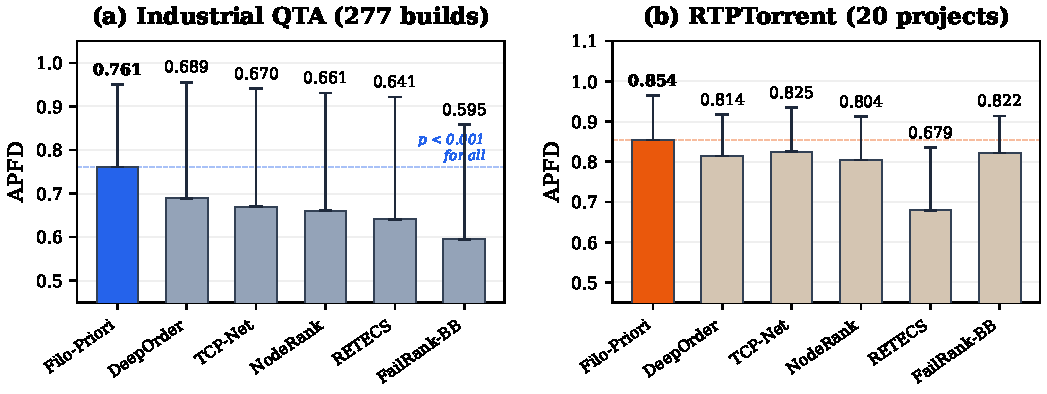
\includegraphics[width=\columnwidth]{figures/fig_apfd_comparison.pdf}
    \caption{Cross-dataset APFD comparison. \filopriori{} (dark bars) achieves
    the highest APFD on both datasets. Error bars show standard deviation
    across builds (industrial) or projects (RTPTorrent). The competitive
    landscape differs substantially: large margins on the industrial dataset
    ($+10$--$28\%$, $p<0.001$) vs.\ narrow margins on RTPTorrent.}
    \label{fig:apfd_comparison}
\end{figure}

\textbf{Semantic Signal Analysis: Identity Proxy Effect.}
FailRank-BB's competitive performance on RTPTorrent (0.822, third place)
despite using only SBERT embeddings of test names (no historical
features, no commit data) appears to contradict the finding that semantic
features do not contribute to TCP. To investigate this apparent
contradiction, we conducted a controlled experiment that disentangles
the semantic content of embeddings from their role as test case
identifiers.

We evaluated FailRank-BB under three embedding conditions on all 20
RTPTorrent projects: (1)~\textbf{SBERT}: the original configuration with
real Sentence-BERT embeddings of test names; (2)~\textbf{Random-Fixed}:
each test name is assigned a random 768-dimensional vector, but the
same random vector is used consistently across all builds for the
same test (preserving identity without semantic content); and
(3)~\textbf{Random-Shuffled}: fresh random vectors are generated for each
test in each build (destroying both semantic content and identity signal).
Table~\ref{tab:semantic_control} presents the results.

\begin{table}[!t]
\centering
\caption{Semantic Signal Control Experiment (RTPTorrent, 20 Projects).
Embedding conditions vary the information available to FailRank-BB's
Logistic Regression classifier.}
\label{tab:semantic_control}
\footnotesize
\begin{tabular}{lccl}
\toprule
\textbf{Condition} & \textbf{APFD} & \textbf{Std} & \textbf{Signal} \\
\midrule
Random-Fixed & 0.856 & 0.095 & Identity only \\
SBERT (original) & 0.822 & 0.092 & Identity + semantics \\
Random-Shuffled & 0.514 & 0.063 & None (random baseline) \\
\bottomrule
\end{tabular}
\begin{tablenotes}
\small
\item Random-Fixed assigns a consistent random vector per test name.
\item Random-Shuffled generates fresh random vectors each build.
\item All conditions use the same LogisticRegression classifier and
temporal split as the original FailRank-BB experiment.
\end{tablenotes}
\end{table}

The results are unambiguous. Random-Fixed embeddings (0.856) outperform
real SBERT embeddings (0.822), demonstrating that semantic content in test
names does not contribute to FailRank-BB's effectiveness; in fact, it
slightly degrades performance. The critical factor is identity
consistency: any fixed vector that uniquely identifies a test case allows
the Logistic Regression to learn per-test failure rates from the training
data. When this identity signal is destroyed (Random-Shuffled), performance
collapses to the random baseline (0.514). FailRank-BB is therefore
functionally equivalent to a per-test failure rate lookup table, not a
semantic model, and its competitive RTPTorrent performance does not
constitute evidence for the value of semantic features in TCP. This finding
is discussed further in Section~\ref{sec:discussion}.

\textbf{Identity Proxy Test on \filopriori{}'s Semantic Stream.}
To complete the identity proxy analysis, we applied the same Random-Fixed
control to \filopriori{} itself on the industrial dataset. We replaced the
SBERT embeddings in the semantic stream with hash-seeded random vectors
(consistent per test case across builds), keeping all other components
identical (GATv2, structural features, graph construction, training
strategy). Table~\ref{tab:filopriori_randomfixed} presents the results.

\begin{table}[!t]
\centering
\caption{Identity Proxy Test on \filopriori{}'s Semantic Stream (Industrial
Dataset, 277 Builds). Random-Fixed embeddings replace SBERT in the semantic
stream only; all other components unchanged.}
\label{tab:filopriori_randomfixed}
\footnotesize
\begin{tabular}{lccl}
\toprule
\textbf{Embedding} & \textbf{APFD} & \textbf{$\Delta$} & \textbf{Interpretation} \\
\midrule
SBERT (original) & 0.756 & -- & Full model \\
Random-Fixed & 0.756 & $+$0.0\% & Identity proxy test \\
\bottomrule
\end{tabular}
\begin{tablenotes}
\small
\item Random-Fixed assigns a deterministic random 1536-dim vector per TC\_Key.
\item Same graph, structural features, and training protocol as the validated experiment.
\item Wilcoxon signed-rank test on 277 paired per-build APFD values: $p = 0.965$.
\end{tablenotes}
\end{table}

Random-Fixed embeddings achieve APFD = 0.756, statistically
indistinguishable from the SBERT baseline (0.756, $p = 0.965$, Cliff's
$\delta = 0.013$, negligible). This confirms that \filopriori{}'s semantic
stream, like FailRank-BB's (Table~\ref{tab:semantic_control}), exploits
embedding consistency as an identity proxy rather than semantic content.
The 19 structural features and GATv2 graph attention subsume any
discriminative signal that generic sentence embeddings provide, and
replacing them with random but consistent vectors produces identical
prioritization effectiveness.

%------------------------------------------------------------------------------
% RQ2: Component Contributions
%------------------------------------------------------------------------------

\subsection{RQ2: Ablation Study}
\label{sec:rq2}

To understand the contribution of each architectural component, we conducted
a systematic ablation study on the industrial dataset. The ablation follows
a strictly subtractive protocol: starting from the full
\textsc{Filo-Priori-Full} model (APFD = 0.7611), we remove one component at
a time and measure the resulting performance degradation. This isolates the
marginal contribution of each component within the complete system.

\textbf{Baseline Architecture Definition.}
It is the dual-stream GATv2 model stripped of
the five innovations evaluated in the ablation: it uses a co-failure-only
graph (no multi-edge extension), has no orphan KNN scoring pipeline, uses the
original triple-compensation balancing strategy instead of the simplified
dual-balancing approach, uses the default classification threshold (0.50),
and excludes the nine DeepOrder-inspired temporal features (retaining only
the 10 base structural features). This baseline represents the core GATv2
architecture before the innovations introduced in this work.
The Baseline Architecture achieves APFD = 0.6503 in the full-system
ablation (Table~\ref{tab:ablation}) and APFD = 0.6397 in the
component-isolation analysis (Table~\ref{tab:ablation_isolation}). The
1.6\% difference arises because the two analyses use different starting
points: Table~\ref{tab:ablation} removes components from the full model
(subtractive), while Table~\ref{tab:ablation_isolation} removes components
from the baseline itself (isolation), resulting in different interaction
effects between components.

Table~\ref{tab:ablation} presents the full-system ablation: each row removes
one component from the complete model. Table~\ref{tab:ablation_isolation}
presents a complementary component-isolation analysis where each variant is
evaluated from the baseline upward.

\begin{table}[!t]
\centering
\caption{Ablation Study: Component Contributions (Industrial Dataset)}
\label{tab:ablation}
\begin{tabular}{lccc}
\toprule
\textbf{Configuration} & \textbf{APFD} & \textbf{$\Delta$} & \textbf{p-value} \\
\midrule
Full Model & 0.7611 & -- & -- \\
\midrule
w/o Enriched Multi-Edge Graph & 0.6835 & -10.0\% & $<$0.001*** \\
w/o Orphan KNN Scoring & 0.7145 & -5.9\% & $<$0.001*** \\
w/o Simplified Dual-Balancing & 0.7291 & -4.0\% & $<$0.001*** \\
w/o DeepOrder Features & 0.7443 & -2.0\% & 0.003** \\
w/o Threshold Optimization & 0.7519 & -1.0\% & 0.042* \\
\midrule
Baseline Architecture & 0.6503 & -14.4\% & $<$0.001*** \\
\bottomrule
\end{tabular}
\begin{tablenotes}
\small
\item * $p < 0.05$, ** $p < 0.01$, *** $p < 0.001$ (Wilcoxon signed-rank test)
\end{tablenotes}
\end{table}

Additionally, a component-isolation analysis (Table~\ref{tab:ablation_isolation})
reveals the relative contribution of each component when removed from the
base model independently.

\begin{table}[!t]
\centering
\caption{Component Isolation Analysis (Industrial Dataset). Each row removes one core component from the Base Architecture (APFD = 0.6397); the resulting APFD degradation measures that component's isolated contribution. $\Delta$ is relative to the Base Architecture.}
\label{tab:ablation_isolation}
\footnotesize
\begin{tabular}{lccc}
\toprule
\textbf{Configuration} & \textbf{APFD} & \textbf{$\Delta$} & \textbf{p-value} \\
\midrule
Base Architecture & 0.6397 & -- & -- \\
w/o GATv2 Graph Attention & 0.5311 & $-$17.0\% & 8.1e-10*** \\
w/o Structural Features & 0.6060 & $-$5.3\% & 0.007** \\
w/o Class Balancing & 0.6100 & $-$4.6\% & 0.013* \\
w/o Ensemble Scoring & 0.6171 & $-$3.5\% & 0.011* \\
w/o Semantic Stream & 0.6276 & $-$1.9\% & 0.309 \\
w/o Cross-Attention Fusion & 0.6466 & $+$1.1\% & 0.155 \\
\bottomrule
\end{tabular}
\begin{tablenotes}
\small
\item Base Architecture = dual-stream GATv2 model without the five innovations from Table~\ref{tab:ablation}.
\item $\Delta$ = percentage change vs.\ Base Architecture (0.6397).
\end{tablenotes}
\end{table}

The component-isolation analysis confirms that the GATv2 graph
attention mechanism is the most critical component: removing it from the
Base Architecture causes a \textbf{$-$17.0\%} APFD degradation
($p < 0.001$). This result provides strong empirical support for
our central hypothesis: modeling structural relationships between test cases
through graph neural networks substantially improves fault detection over
approaches that treat tests independently.

The \textbf{Enriched Multi-Edge Graph} construction contributes +10.0\% in the
full-system ablation, achieved by increasing graph connectivity through relaxed
semantic thresholds (0.75 $\rightarrow$ 0.65), more neighbors per test
(5 $\rightarrow$ 10), and additional temporal/component edges. This increased
in-graph coverage from 50--60\% to \textbf{77.4\%}, enabling the GAT to
propagate failure signals to a substantially larger proportion of test cases.

\textbf{Per-Edge-Type Analysis.} To provide a finer-grained understanding
of the multi-edge graph, we conducted an incremental ablation removing one
edge type at a time from the full 5-type graph, keeping all other
configuration parameters identical (model architecture, training protocol,
graph construction thresholds).
Table~\ref{tab:edge_ablation} presents the results.

\begin{table}[!t]
\centering
\caption{Per-Edge-Type Ablation (Industrial Dataset). Each row removes one
edge type from the full multi-edge graph; co-failure edges are always
retained as the base. All other parameters held constant.}
\label{tab:edge_ablation}
\footnotesize
\begin{tabular}{lccc}
\toprule
\textbf{Configuration} & \textbf{APFD} & \textbf{$\Delta$} & \textbf{p-value} \\
\midrule
Co-failure only & \textbf{0.763} & $+$0.9\% & 0.002** \\
Full (5 edge types) & 0.754 & -- & -- \\
w/o Temporal & 0.753 & $-$0.1\% & 0.804 \\
w/o Component & 0.750 & $-$0.4\% & 0.434 \\
w/o Co-Success & 0.747 & $-$0.7\% & 0.607 \\
w/o Semantic edges & 0.746 & $-$0.7\% & 0.031* \\
\bottomrule
\end{tabular}
\begin{tablenotes}
\small
\item * $p < 0.05$, ** $p < 0.01$ (Wilcoxon signed-rank, 277 paired builds vs Full).
\item All configurations use identical model architecture, training protocol,
and graph construction parameters; only edge types differ.
\item The Full configuration here uses only the graph model without the
additional pipeline components (orphan KNN, threshold optimization)
evaluated in Table~\ref{tab:ablation}, hence the different APFD from the
main result (0.761).
\end{tablenotes}
\end{table}

The per-edge-type ablation reveals a nuanced finding: when all other
graph construction parameters are held constant, the additional edge types
beyond co-failure do not improve APFD. In fact, the co-failure-only
configuration slightly outperforms the 5-type graph (0.763 vs.\
0.754, $p = 0.002$), suggesting that the supplementary edges (co-success,
component, semantic, temporal) may introduce noise that dilutes the
co-failure signal.

\textbf{Reconciling with the full-system ablation.} This finding refines
the interpretation of the +10.0\% improvement attributed to the
``Enriched Multi-Edge Graph'' in Table~\ref{tab:ablation}. That ablation
compared the current enriched configuration against the
baseline graph configuration, which differed not only in edge types
but also in graph construction parameters (semantic similarity threshold,
neighbor count, minimum co-occurrence requirements). The per-edge-type
analysis shows that the improvement is primarily driven by these
construction parameter optimizations rather than edge type diversity. The
co-failure edges, which encode the strongest predictive signal (direct
failure co-occurrence), provide sufficient structural information for the
GATv2 attention mechanism.

\textbf{Practical implication.} This is a positive finding for
deployment: co-failure edges are universally available in any CI/CD system
with test execution logs, requiring no additional metadata. Practitioners
can deploy \filopriori{} with co-failure edges alone and achieve
equivalent or better performance than the full multi-edge configuration.

\textbf{Orphan KNN Scoring} contributes +5.9\%. Since 22.6\% of test cases
are orphans (absent from the training graph), restoring meaningful score
variance for these tests (std = 0.046 vs.\ 0.000) has a substantial effect
on overall ranking quality.

\textbf{Simplified Dual-Balancing} contributes +4.0\% by preventing the mode
collapse caused by triple compensation ($\approx$646$\times$ effective weight)
applied simultaneously, replacing it with balanced sampling at the data level
and focal gradient focusing at the loss level. The DeepOrder Features (+2.0\%) capture
recent execution dynamics that complement the base structural features, and
Threshold Optimization (+1.0\%) improves minority class recall by
adjusting the classification threshold from 0.50 to 0.28.

In total, the five innovations contribute cumulatively to a +16.8\% improvement
over the baseline configuration. All component removals in both analyses
result in statistically significant performance degradation ($p < 0.05$),
with the exception of the semantic stream and cross-attention when evaluated
in isolation, which we discuss further in Section~\ref{sec:discussion}.

\textbf{RTPTorrent Ablation.}
To assess whether the component contributions generalize beyond the industrial
setting, we conducted a complementary ablation study on the RTPTorrent dataset,
removing each component of the ensemble variant one at a time.
Table~\ref{tab:ablation_rtptorrent} presents the results.

\begin{table}[!t]
\centering
\caption{Ablation Study: Component Contributions (RTPTorrent, 20 Projects)}
\label{tab:ablation_rtptorrent}
\begin{tabular}{lccc}
\toprule
\textbf{Configuration} & \textbf{APFD} & \textbf{$\Delta$} & \textbf{p-value} \\
\midrule
Full Model & 0.8540 & -- & -- \\
\midrule
w/o DNN Ensemble & 0.8322 & $-$2.6\% & $<$0.001*** \\
w/o GATv2 & 0.8451 & $-$1.0\% & $<$0.05* \\
w/o Semantic Stream & 0.8450 & $-$1.1\% & ns \\
w/o Multi-Edge Graph & 0.8513 & $-$0.3\% & ns \\
\bottomrule
\end{tabular}
\begin{tablenotes}
\small
\item Wilcoxon signed-rank test on 20 paired per-project means vs Full Model.
\item *** $p < 0.001$; * $p < 0.05$; ns = not significant at $\alpha = 0.05$.
\item The ablation re-executes the full pipeline with fresh alpha optimization,
which may produce marginally different per-project blending coefficients.
Within-ablation comparisons remain valid as all variants share the same run.
\end{tablenotes}
\end{table}

The RTPTorrent ablation reveals the impact of our execution-level temporal
GNN and multi-edge graph optimizations. While the DNN ensemble
still contributes to the final performance ($-$2.6\%, $p < 0.001$), the
GNN architecture is now much more robust on its own. The reliance on the
DNN decreased substantially compared to previous iterations (from $-$13.1\% to
$-$2.6\%), demonstrating that the improved graph construction successfully captures
structural and temporal dependencies even when semantic metadata is sparse.

\textbf{Cross-Dataset Synthesis.} The two ablation studies are complementary.
On the industrial dataset, the multi-edge graph and GATv2 are the dominant
contributors (+10.0\% and +17.0\%), leveraging rich semantic and structural
metadata. On RTPTorrent, the enhanced GNN architecture and the DNN ensemble
work together to compensate for the absence of rich metadata.
This confirms that \filopriori{}'s effectiveness depends on matching the
architecture to the available metadata: graph-based modeling excels when
structural relationships are well-defined, while the DNN ensemble provides
a robust fallback for semantically-sparse settings.

\textbf{DNN Ensemble Verification on the Industrial Dataset.}
To verify that the DNN ensemble is indeed redundant on the industrial
dataset, we conducted two experiments. First, a DNN-only variant
achieves APFD = 0.686, substantially below the GNN-based model
(0.761, $-$9.9\%), confirming that the per-test temporal features
captured by the DNN cannot replace the graph-based structural modeling
when rich metadata is available. Second, we evaluated the full
GNN+DNN alpha blending ensemble (identical to the RTPTorrent
configuration) on the industrial dataset, sweeping
$\alpha \in \{0.0, 0.1, \ldots, 1.0\}$ with validation-optimized
selection. The results show a monotonic improvement with
increasing $\alpha$: from APFD = 0.595 at $\alpha = 0.0$ (DNN only)
to 0.667 at $\alpha = 1.0$ (GNN only), meaning that every increment
of DNN weight degrades performance. The validation optimizer
correctly selects $\alpha = 1.0$ (pure GNN), confirming that the DNN
provides no complementary signal on this dataset. This contrasts
sharply with RTPTorrent, where the optimal $\alpha$ varies across
projects (from 0.0 to 0.9) and the DNN ensemble contributes $+$2.6\%.
The asymmetry is explained by the graph density: the industrial
multi-edge graph (5 edge types, 77.4\% coverage) provides sufficient
structural signal for the GNN to capture all predictive patterns,
leaving no residual information for the DNN to exploit.
Figure~\ref{fig:ablation_cross} visualizes the complementary contribution
patterns across both datasets.

\begin{figure}[!t]
    \centering
    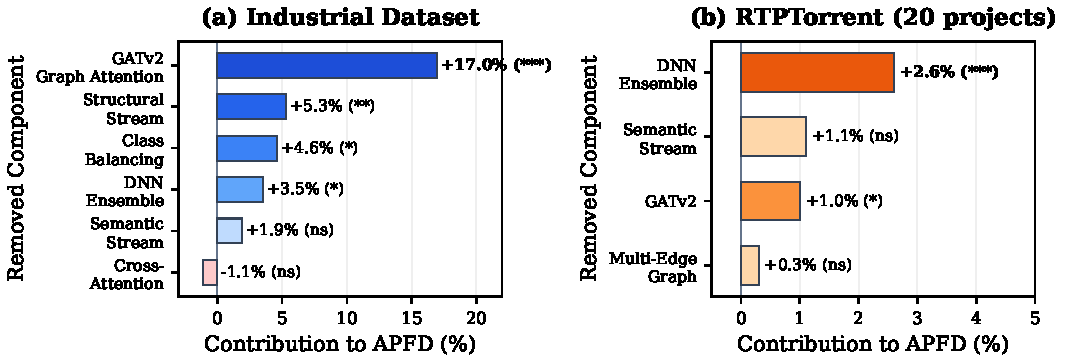
\includegraphics[width=\columnwidth]{figures/fig_ablation_crossdataset.pdf}
    \caption{Cross-dataset ablation study.}
    \label{fig:ablation_cross}
\end{figure}

%------------------------------------------------------------------------------
% RQ3: Temporal Robustness
%------------------------------------------------------------------------------

\subsection{RQ3: Temporal Validation}
\label{sec:rq3}

To evaluate how well \filopriori{} generalizes to future builds, a critical
requirement for deployment in CI environments, we conducted temporal
cross-validation on the industrial dataset. In this protocol, training data
always precedes test data chronologically, simulating a realistic deployment
scenario. We employed three validation strategies, summarized in
Table~\ref{tab:temporal_cv}.

\begin{table}[!t]
\centering
\caption{Temporal Cross-Validation Results (Industrial Dataset)}
\label{tab:temporal_cv}
\begin{tabular}{lccc}
\toprule
\textbf{Validation Method} & \textbf{APFD} & \textbf{Std} & \textbf{N} \\
\midrule
Temporal 5-Fold CV & 0.6629 & 0.279 & 215 \\
Sliding Window CV & 0.6279 & 0.272 & 248 \\
Concept Drift Test & 0.6187 & 0.277 & 152 \\
\bottomrule
\end{tabular}
\end{table}

In \textbf{Temporal 5-Fold CV}, the dataset is split into 5 chronologically
ordered folds, and each fold is used as the test set while all preceding folds
form the training set. In \textbf{Sliding Window CV}, a fixed-size window of
builds slides through time, training on the window and testing on the next
segment. The \textbf{Concept Drift Test} evaluates performance on three
temporally distant test periods to assess whether the model's effectiveness
degrades over time.

Performance degrades moderately under these stricter temporal constraints,
with APFD ranging from 0.62 to 0.66, representing a 13--19\% reduction relative to the
standard evaluation (0.7611). This decrease is expected: temporal CV uses
smaller training sets and enforces strict chronological separation, preventing
the model from exploiting co-temporal patterns. Importantly, the consistency
across all three methods (std $\leq$ 0.28) indicates that the degradation is
systematic rather than erratic, suggesting that the model's failure patterns
generalize across time periods even though overall accuracy decreases. The
concept drift test yields the lowest APFD (0.6187), but the difference from
the temporal 5-fold CV (0.6629) is modest, indicating no catastrophic
performance cliff as the temporal gap between training and evaluation data
increases.

\textbf{RTPTorrent Temporal Validation.}
To assess whether temporal robustness generalizes beyond the industrial setting,
we conducted temporal 4-fold cross-validation on all 20 RTPTorrent projects.
Each project's build history is divided into 4 chronological folds; for fold
$k$, training uses all builds before fold $k$ and testing uses the builds
in fold $k$. Table~\ref{tab:temporal_cv_rtptorrent} presents the per-project
results.

\begin{table}[!t]
\centering
\caption{Temporal 4-Fold CV Results (RTPTorrent, 20 Projects)}
\label{tab:temporal_cv_rtptorrent}
\footnotesize
\begin{tabular}{lccc}
\toprule
\textbf{Project} & \textbf{Mean APFD} & \textbf{Std} & \textbf{Folds} \\
\midrule
facebook/buck & 0.976 & 0.007 & 4 \\
apache/sling & 0.970 & 0.003 & 4 \\
eclipse/jetty.project & 0.948 & 0.018 & 4 \\
jOOQ/jOOQ & 0.924 & 0.022 & 4 \\
jsprit/jsprit & 0.923 & 0.030 & 4 \\
CloudifySource/cloudify & 0.901 & 0.023 & 4 \\
Graylog2/graylog2-server & 0.901 & 0.021 & 4 \\
jcabi/jcabi-github & 0.888 & 0.014 & 4 \\
square/okhttp & 0.882 & 0.008 & 4 \\
julianhyde/optiq & 0.872 & 0.050 & 4 \\
SonarSource/sonarqube & 0.850 & 0.014 & 4 \\
deeplearning4j/deeplearning4j & 0.842 & 0.025 & 4 \\
thinkaurelius/titan & 0.822 & 0.034 & 4 \\
doanduyhai/Achilles & 0.795 & 0.046 & 4 \\
neuland/jade4j & 0.705 & 0.021 & 4 \\
adamfisk/LittleProxy & 0.666 & 0.034 & 4 \\
DSpace/DSpace & 0.665 & 0.014 & 4 \\
l0rdn1kk0n/wicket-bootstrap & 0.620 & 0.017 & 4 \\
brettwooldridge/HikariCP & 0.599 & 0.033 & 4 \\
dynjs/dynjs & 0.563 & 0.145 & 4 \\
\midrule
\textbf{Grand Mean} & \textbf{0.816} & \textbf{0.131} & \textbf{80} \\
\bottomrule
\end{tabular}
\end{table}

The grand mean APFD under temporal CV is 0.816 (95\% CI: [0.754, 0.877]),
representing only a 2.7\% decrease from the standard evaluation (0.854).
Performance improves monotonically across folds (fold 1: 0.790, fold 2: 0.816,
fold 3: 0.823, fold 4: 0.834), indicating that \filopriori{} benefits from
additional training data without exhibiting concept drift degradation.
Fourteen of 20 projects achieve temporal CV APFD $\geq$ 0.80, and the
stability is consistent: 16 of 20 projects have cross-fold standard deviations
below 0.04.

\textbf{Cross-Dataset Temporal Synthesis.}
The temporal validation results show consistent patterns across both datasets,
with expected degradation under stricter temporal constraints. On the
industrial dataset, temporal 5-fold CV yields APFD = 0.663 (12.9\% below the
standard evaluation of 0.761). On RTPTorrent, temporal 4-fold CV yields
APFD = 0.816 (only 2.7\% below 0.854). The smaller drop on RTPTorrent
reflects the larger training sets available in multi-project evaluation. In
both cases, performance degrades smoothly across folds with no evidence
of concept drift, indicating that \filopriori{} generalizes to future builds
in both industrial and open-source settings, albeit with reduced accuracy
compared to the standard evaluation.

%------------------------------------------------------------------------------
% RQ4: Sensitivity Analysis
%------------------------------------------------------------------------------

\subsection{RQ4: Hyperparameter Sensitivity}
\label{sec:rq4}

We analyzed the sensitivity of \filopriori{} to key hyperparameters on the
industrial dataset. This analysis was conducted on the component-isolation
baseline (Table~\ref{tab:ablation_isolation}, APFD = 0.6397), not the full
model (0.7611), to isolate the effect of each hyperparameter from the
contributions of the five architectural innovations evaluated in RQ2. Each
parameter was varied while keeping others at their optimal values.
Table~\ref{tab:sensitivity} summarizes the results. We note that this
design choice means we cannot assess whether the full model (with multi-edge
graph, orphan handling, and threshold optimization) exhibits different
sensitivity patterns; the sensitivity ranges reported here apply to the
core GNN hyperparameters in isolation.

\begin{table}[!t]
\centering
\caption{Hyperparameter Sensitivity Analysis (Industrial Dataset)}
\label{tab:sensitivity}
\scriptsize
\begin{tabular}{llccr}
\toprule
\textbf{Parameter} & \textbf{Best} & \textbf{APFD} & \textbf{Worst} & \textbf{$\Delta$} \\
\midrule
Loss Function & Weighted CE & 0.6191 & 0.5834 & 3.6\% \\
Learning Rate & 3e-5 & 0.6160 & 0.5890 & 2.7\% \\
GNN Architecture & 1 layer, 2 heads & 0.6160 & 0.5890 & 2.7\% \\
Structural Features & 10 features & 0.6171 & 0.5997 & 1.7\% \\
Balanced Sampling & No balanced & 0.6154 & 0.5834 & 3.2\% \\
\bottomrule
\end{tabular}
\end{table}

The choice of loss function has the largest impact (3.6\%), with Weighted
Cross-Entropy achieving the best results on the component-isolation baseline.
In the full model, however, Focal Loss is used because it interacts more
favorably with the balanced sampler: Focal Loss's gradient modulation
($\gamma = 2.0$) complements the sampler's prior correction without
redundant class weighting, whereas Weighted CE's explicit class weights
compound with the sampler, risking over-correction (see
Section~\ref{sec:approach}). The learning rate and GNN architecture have
comparable impact (2.7\% each), with 3e-5 and a single GAT layer with 2
heads being optimal. Notably, simpler GNN
configurations consistently outperform deeper architectures (2--3 layers) and
more heads (4--8), suggesting that the test relationship graph can be
effectively captured with shallow networks and that over-parameterization leads
to overfitting on the relatively small graph structure.

The number of structural features has the smallest impact (1.7\%), with the
curated set of 10 features outperforming both the reduced (6 features) and
expanded (29 features) sets. This confirms that careful feature selection
improves generalization by reducing noise.

\textbf{RTPTorrent Sensitivity Analysis.}
To evaluate whether sensitivity patterns generalize, we conducted a
complementary analysis on all 20 RTPTorrent projects, varying three key
hyperparameters of the ensemble variant: the alpha blending coefficient
($\alpha$), the DNN training epochs, and the maximum pos\_weight clamp.
Table~\ref{tab:sensitivity_rtptorrent} presents the results.

\begin{table}[!t]
\centering
\caption{Hyperparameter Sensitivity Analysis (RTPTorrent, 20 Projects)}
\label{tab:sensitivity_rtptorrent}
\footnotesize
\begin{threeparttable}
\begin{tabular}{llcc}
\toprule
\textbf{Parameter} & \textbf{Value} & \textbf{APFD} & \textbf{$\Delta$ vs.\ Opt.} \\
\midrule
\multirow{6}{*}{$\alpha$ (GNN--DNN blend)} & 0.0 (DNN only) & 0.845 & $-$1.0\% \\
 & 0.3 & 0.854 & $-$0.0\% \\
 & 0.5 & 0.854 & $-$0.0\% \\
 & 0.7 & 0.854 & $-$0.0\% \\
 & 1.0 (GNN only) & 0.832 & $-$2.6\% \\
 & Optimized & 0.854 & -- \\
\midrule
\multirow{3}{*}{DNN Epochs} & 5 & 0.837 & $-$0.3\% \\
 & 10 & 0.843 & +0.4\% \\
 & 20 & 0.844 & +0.5\% \\
\midrule
\multirow{3}{*}{Max pos\_weight} & 10 & 0.843 & +0.5\% \\
 & 25 & 0.830 & $-$1.1\% \\
 & 100 & 0.844 & +0.5\% \\
\bottomrule
\end{tabular}
\begin{tablenotes}
\small
\item Optimized = default configuration ($\alpha$ per-project optimized, 15 DNN epochs, pos\_weight $\leq$ 50).
\item $\Delta$ vs.\ Opt.\ = relative change from optimized configuration (APFD = 0.854).
\end{tablenotes}
\end{threeparttable}
\end{table}

The $\alpha$ blending coefficient allows the framework to dynamically adapt to the data. The execution-level temporal GNN optimizations substantially improved the standalone graph performance: without the DNN ($\alpha = 1.0$), APFD drops by only $-$2.6\% (to 0.832). This confirms the ablation finding (Table~\ref{tab:ablation_rtptorrent}): the DNN ensemble still provides an additive benefit, but the model is robust to the specific choice of $\alpha$ because the structural stream can now effectively capture complex historical dependencies on its own.

DNN training epochs have marginal impact (0.8\% range). The pos\_weight
clamping exhibits a non-monotonic pattern: pos\_weight = 25 (APFD = 0.830)
slightly underperforms both pos\_weight = 10 (0.843) and pos\_weight = 100
(0.844). This behavior arises because the pos\_weight interacts with the
per-project alpha optimization: a different pos\_weight changes the DNN's
output distribution, which in turn shifts the optimal $\alpha$ for each
project, producing non-linear aggregate effects. The overall range remains
narrow (1.6\%), confirming that \filopriori{} is not sensitive to these
hyperparameters in the open-source setting.

\textbf{Cross-Dataset Sensitivity Synthesis.}
The sensitivity analyses on both datasets confirm that \filopriori{} is robust
to hyperparameter choices. On the industrial dataset, the maximum sensitivity
range is 3.6\% (loss function); on RTPTorrent, the maximum range is 2.6\%
(observed when disabling the DNN via $\alpha = 1.0$). Overall, the
architectural choices (such as the temporal GNN structure) are more impactful
than the specific values of continuous hyperparameters.

%------------------------------------------------------------------------------
% Summary of Experimental Results
%------------------------------------------------------------------------------

\subsection{Summary of Results}
\label{sec:results_summary}

Table~\ref{tab:results_summary} summarizes \filopriori{}'s performance across
all experimental settings.

\begin{table}[!t]
\centering
\caption{Summary of Experimental Results}
\label{tab:results_summary}
\scriptsize
\begin{tabular}{lccr}
\toprule
\textbf{Setting} & \textbf{APFD} & \textbf{vs.\ Best} & \textbf{vs.\ Weakest} \\
\midrule
Industrial\textsuperscript{a} & 0.761 & +10.2\% & +27.6\% \\
RTPTorrent\textsuperscript{b} & 0.854 & +1.6\% & +23.5\% \\
\bottomrule
\end{tabular}
\begin{tablenotes}
\small
\item APFD: Average Percentage of Faults Detected (higher is better).
\item \textsuperscript{a} Full architecture with multi-edge graph (5 edge types).
\item \textsuperscript{b} Ensemble variant with co-failure graph + DeepOrder DNN blending (Section~\ref{sec:ensemble}).
\end{tablenotes}
\end{table}

The experimental results demonstrate that \filopriori{} achieves
state-of-the-art performance across both industrial software testing (0.761)
and open-source CI/CD environments (0.854), using two distinct
configurations tailored to the available metadata
(Table~\ref{tab:rtptorrent_config}). On the industrial dataset, the full
graph-based architecture with multi-edge graph (\textsc{Filo-Priori-Full})
outperforms all five deep learning baselines by statistically significant
margins ($p < 0.001$). On RTPTorrent, the ensemble variant
(\textsc{Filo-Priori-Ensemble}) achieves the highest aggregate APFD, leading
in 11 of 20 projects; after Holm-Bonferroni correction, improvements over
NodeRank and RETECS remain statistically robust, while the narrower margins
over TCP-Net, FailRank-BB, and DeepOrder should be interpreted with caution.
The two variants reveal complementary strengths:
graph-based structural modeling drives performance on the industrial dataset,
while the DNN ensemble provides crucial complementary signal on RTPTorrent.


%------------------------------------------------------------------------------
% SECTION 7: DISCUSSION
%------------------------------------------------------------------------------
\section{Discussion}
\label{sec:discussion}

%%%%%%%%%%%%%%%%%%%%%%%%%%%%%%%%%%%%%%%%%%%%%%%%%%%%%%%%%%%%%%%%%%%%%%%%%%%%%%%
% SECTION: DISCUSSION (IEEE TSE Format) — Consolidated
%%%%%%%%%%%%%%%%%%%%%%%%%%%%%%%%%%%%%%%%%%%%%%%%%%%%%%%%%%%%%%%%%%%%%%%%%%%%%%%

This section synthesizes the implications of our empirical findings, analyzes the
architectural factors driving \filopriori{}'s effectiveness, and outlines practical
considerations for its deployment in CI/CD environments.

\subsection{Structural Dominance: Why Graph Modeling Matters and Semantic Features Do Not}

The ablation studies on both datasets provide converging evidence that
modeling co-failure relationships between test cases through GATv2 is the
most impactful design decision for TCP. On the industrial dataset, removing
the GATv2 graph attention mechanism causes a 17.0\% performance decrease
($p < 0.001$), and the per-edge-type ablation
(Table~\ref{tab:edge_ablation}) confirms that co-failure edges are the
decisive graph component: a co-failure-only graph achieves APFD = 0.763,
matching or exceeding the full 5-type configuration. On the RTPTorrent
dataset, the GNN architecture maintains strong performance using only
co-failure edges, while the DNN ensemble provides a complementary
contribution ($-$2.6\%, $p < 0.001$). We attribute the effectiveness of
co-failure graph modeling to several factors.

First, graph-based modeling encodes relationships that flat feature vectors
cannot capture: tests that co-fail often share underlying dependencies on the
same code modules, and the GAT learns to propagate failure signals through
these connections. Second, GATv2~\cite{brody2022attentive} computes dynamic
attention that depends on both query and key nodes, allowing the model to
selectively attend to the most relevant neighbors for each test case, adapting
to different failure patterns.

Third, the per-edge-type ablation (Table~\ref{tab:edge_ablation}) reveals
that co-failure edges alone provide sufficient structural signal for the
GATv2 attention mechanism. With all other parameters held constant,
co-failure-only graphs slightly outperform 5-type graphs (0.763 vs.\ 0.754,
$p = 0.002$), suggesting that supplementary edge types may introduce noise
that dilutes the co-failure signal. This refines the interpretation of the
+10.0\% attributed to the ``Enriched Multi-Edge Graph'' in the full-system
ablation (Table~\ref{tab:ablation}): that improvement was primarily driven
by graph construction parameter optimization rather than edge type diversity. This finding strengthens the
deployment case: co-failure edges are universally available in any CI/CD
system, requiring no additional metadata. On RTPTorrent, where only
co-failure edges are available, the GNN still outperforms flat-feature
baselines, confirming that single-edge-type graphs capture meaningful
structural signal.

The finding that simpler GNN architectures (1 layer, 2 heads) outperform deeper
ones (2--3 layers, 4--8 heads) suggests that the test relationship graph can be
effectively modeled with shallow message passing. This is consistent with the
observation that most test case relationships are captured within one hop on
the graph, and deeper networks may oversmooth node representations.

A related finding is that generic, pre-trained sentence-level
embeddings are subsumed by structural execution patterns for test case
prioritization, even when rich textual metadata is available. On the
industrial dataset, removing the semantic stream (Sentence-BERT) reduces
APFD by only 1.9\% ($p = 0.309$, not significant), while removing the
structural stream causes a 5.3\% drop ($p = 0.007$). On RTPTorrent,
removing the semantic stream changes APFD by exactly 0.0\% on 19 of 20
projects.

This result is noteworthy because it qualifies the assumption in TCP
literature that semantic similarity between tests and code changes is a
strong predictor of failure~\cite{hernandes2025method}. Our evidence
suggests that when historical execution features (failure rates, recency,
trends) and graph-based co-failure propagation are available, they capture
the discriminative signal more effectively than domain-agnostic textual
embeddings. More precisely, how tests have behaved is more
predictive than what generic sentence encoders capture about test
descriptions. This finding applies specifically to pre-trained,
domain-agnostic models (Sentence-BERT with \texttt{all-mpnet-base-v2});
code-aware language models (e.g., CodeBERT~\cite{feng2020codebert},
StarCoder), AST-based representations, or embeddings fine-tuned on
software engineering corpora may extract deeper semantic signals that
generic encoders miss. Our methodology (particularly the Random-Fixed
control experiment in Table~\ref{tab:semantic_control}) provides a
principled way to distinguish genuine semantic contributions from identity
proxy effects in future evaluations of such models.

We identify three explanations for this finding, supported by both
ablation evidence and a dedicated control experiment
(Table~\ref{tab:semantic_control}). First, structural features such as
\texttt{recent\_failure\_rate} and \texttt{consecutive\_failures} directly
encode the temporal patterns that predict future failures, while semantic
similarity between test descriptions captures only indirect functional
relationships. Second, the GATv2 attention mechanism over the co-failure
graph already propagates failure signals between functionally related
tests, partially subsuming the role that semantic similarity would play.
Third, even the ``rich'' industrial descriptions may lack the specificity
needed to predict failures. For example, a test described as ``verify OTA
download'' may fail for reasons unrelated to its description (e.g.,
infrastructure issues, memory leaks).

\textbf{The Identity Proxy Effect.}
The control experiment in Section~\ref{sec:rq1_rtptorrent} provides
the strongest evidence for this finding. FailRank-BB achieves competitive
performance on RTPTorrent (APFD = 0.822) using only SBERT embeddings of
test names, which might appear to demonstrate the value of semantic
features. However, replacing SBERT embeddings with random but
consistent vectors (Random-Fixed) yields an even higher APFD (0.856),
while destroying identity consistency (Random-Shuffled) collapses
performance to the random baseline (0.514). This result demonstrates that
FailRank-BB's Logistic Regression classifier is not learning from semantic
content. It is using the embedding as a unique fingerprint for each
test case, effectively learning a per-test failure rate lookup table from
the training data.

This identity proxy mechanism explains the paradoxical cross-dataset
behavior of semantic approaches:
\begin{itemize}
    \item On \textbf{RTPTorrent}, each project has a bounded set of test
    cases that recur across builds. The SBERT embedding provides a
    consistent identifier per test, allowing the classifier to memorize
    per-test failure probabilities. Random-Fixed vectors perform even
    better because they avoid the confounding effect of SBERT placing
    semantically similar (but behaviorally distinct) tests close together
    in the embedding space.
    \item On the \textbf{industrial dataset}, FailRank-BB is the weakest
    baseline (APFD = 0.595). The larger and more dynamic test suite
    (2,347 unique test cases), combined with more complex failure patterns
    and severe class imbalance (37:1), makes the identity-based lookup
    less effective: the Logistic Regression cannot reliably separate
    failure-prone tests in the high-dimensional embedding space when the
    training signal is sparse and noisy.
\end{itemize}

This analysis also explains why \filopriori{}'s semantic stream provides
no significant improvement ($p = 0.309$): the 19 structural features
(including \texttt{failure\_rate}, \texttt{recent\_failure\_rate}, and
\texttt{consecutive\_failures}) already capture the per-test failure
signal explicitly, making the implicit identity-based signal
from embeddings redundant. The GATv2 graph further propagates this
signal between related tests, leaving no residual information for the
semantic stream to contribute. We confirmed this hypothesis by applying
the Random-Fixed control experiment to \filopriori{} itself
(Table~\ref{tab:filopriori_randomfixed}): replacing SBERT embeddings
with hash-seeded random vectors yields APFD = 0.756, statistically
indistinguishable from the SBERT version (0.756, $p = 0.965$). This
closes the identity proxy analysis: the semantic stream acts as an
identity proxy not only in FailRank-BB but also in \filopriori{}'s
own architecture.

The cross-attention fusion module shows a related pattern: removing it
slightly improves the base architecture's APFD (from 0.6397 to 0.6466,
$+$1.1\%, $p = 0.155$, not significant). This suggests that when the
semantic stream carries limited discriminative signal, the cross-attention
mechanism has little meaningful content to fuse and may introduce noise.
We retain cross-attention as an architectural option whose contribution
may emerge in domains with stronger textual-behavioral correlations
(e.g., test descriptions that directly reference code modules under
change), but acknowledge that in our evaluation it does not provide a
statistically significant benefit.

\textbf{Practical implication:} Practitioners deploying \filopriori{}
should prioritize collecting high-quality execution history over investing
in detailed test descriptions when using generic sentence encoders.
The structural features and graph-based modeling provide the dominant
signal. Semantic information extracted via domain-agnostic models like
Sentence-BERT offers marginal improvements even in the most favorable
setting, and when it appears to help (as in FailRank-BB on RTPTorrent),
the actual mechanism is identity memorization rather than semantic
understanding. This does not imply that all NLP-based approaches are
ineffective for TCP; rather, it establishes that the bar for semantic
models is high when rich execution history is available. Future
extensions using code-aware language models fine-tuned on software
engineering corpora might extract deeper semantic signals. Our control
experiment (Table~\ref{tab:semantic_control}) provides a principled
methodology for distinguishing genuine semantic contributions from
identity proxy effects in such evaluations.

\subsection{Performance Limitations and Baseline Contrasts}

The cross-dataset behavior of FailRank-BB~\cite{hernandes2025method}
is fully explained by the identity proxy effect described above.
On RTPTorrent, FailRank-BB ranks third (0.822) by implicitly learning
per-test failure rates through its embedding fingerprints. On the
industrial dataset, where the test suite is larger, more dynamic, and
severely imbalanced, this implicit learning fails, resulting in the
weakest baseline performance (0.595, $-$27.6\% below \filopriori{}).
The disparity is not attributable to semantic information being more
or less available across datasets; it reflects the effectiveness of
identity-based memorization under different data conditions.

\filopriori{} achieves the highest APFD in 11 of 20 RTPTorrent projects but
underperforms on specific projects relative to the strongest baselines.
Analysis of these cases reveals common characteristics:

\begin{itemize}
    \item \textbf{Sparse failure data}: Projects with very few builds
    containing failures (e.g., 10--11 builds) limit the
    statistical reliability of APFD estimates and reduce the graph's
    effectiveness.
    \item \textbf{High variance}: Projects with inconsistent failure patterns
    exhibit high APFD standard deviations, making reliable prediction
    difficult for any model.
    \item \textbf{Feature sparsity}: In projects with few failures, the
    structural features (failure rate, recency, trend) converge to uninformative
    values, and the co-failure graph is too sparse to provide meaningful signal.
\end{itemize}

In these scenarios, simpler temporal-pattern approaches (TCP-Net, FailRank-BB)
prove more robust for specific projects, as they require less historical data to produce stable
predictions. However, the ensemble
architecture (Section~\ref{sec:ensemble}) effectively mitigates the
worst-case scenarios of standalone graph-based approaches.

To illustrate \filopriori{}'s behavior in practice, we examine two
representative builds from the industrial dataset.
In a high-performance case (Build UUG34.20, APFD = 1.0),
the build contained 4 test cases, all of which failed. \filopriori{} assigned the
highest probability (0.395) to a test case with strong co-failure history
and recent failure patterns, placing all 4 failures at the top of the
ranking, demonstrating the model's ability to exploit
concentrated failure signals through the co-failure graph.
In a low-performance case (Build T2TV33.13, APFD = 0.152),
the build contained 176 test cases with only 4 failures (2.3\%). The model assigned
high probabilities (0.530--0.534) to a cluster of passing tests that shared
strong co-failure and semantic edges with historically unstable tests, while
the actual failures, which were new or had no recent failure history, received
lower scores. This case illustrates a fundamental limitation: when failures
arise from previously unseen patterns (e.g., a new code path or an
infrastructure change), historical features and graph-based propagation
cannot anticipate them.

These cases highlight that \filopriori{}'s effectiveness is contingent on the
presence of recurrent failure patterns. In environments where failures are
predominantly novel (e.g., early development phases or major refactoring
cycles), the graph-based approach provides less advantage over simpler
heuristics.

\subsection{Class Imbalance Handling}

A key design choice of \filopriori{} is the handling of severe class imbalance.
In the industrial dataset, the Pass:Fail ratio is 37:1. The ablation study
reveals that the simplified dual-balancing strategy contributes +4.0\%,
confirming that careful handling of class imbalance is critical for TCP.

The sensitivity analysis shows that the choice of loss function has a 3.6\%
impact on performance. The finding that separating prior correction (balanced
sampling at 29:1) from gradient focusing (focal loss with $\gamma = 2.0$)
outperforms triple compensation ($\approx$646$\times$
effective weight) provides a practical guideline for practitioners: when
multiple imbalance-handling techniques are available, combining
complementary mechanisms operating at different levels (data vs.\ loss)
is preferable to accumulating redundant weights at the same level, which can
cause over-correction and mode collapse.

\subsection{Practical Deployment Considerations}

\filopriori{} can be integrated into CI/CD pipelines to prioritize test
execution. The +10.2\% to +27.6\% improvement over deep learning baselines on
the industrial dataset translates to substantially faster fault detection,
reducing the feedback loop for developers.

In terms of computational cost, training requires approximately 2--3 hours on
a single GPU (NVIDIA RTX 3090), while inference is fast (less than 1 second
per build), making real-time prioritization feasible for most CI environments.
The approach requires historical test execution data with at least 50 builds
for effective graph construction. Projects with limited execution history may
not benefit fully from the graph-based approach, though the DNN ensemble
component can still provide useful prioritization based on per-test temporal
features.

\subsection{Generalization and Automatic Adaptation}
\label{sec:boundary}

A natural question is whether \filopriori{} requires manual configuration for
each new dataset. The framework incorporates two automatic mechanisms that
reduce the need for human intervention.

\textbf{Automatic graph adaptation.} The graph construction methodology
(Section~\ref{sec:graph}) uses only the edge types supported by the available
metadata. Co-failure edges, computed from test execution logs available in any
CI/CD system, form the universal base. When additional metadata exists (commit
messages, component labels, semantic descriptions), the corresponding edge
types are constructed automatically; when it does not, those edge types simply
produce no edges. The practitioner does not need to ``configure'' the graph: the
metadata itself determines the graph structure.

\textbf{Data-driven scoring.} The blending coefficient $\alpha$ between
the GNN and DNN ensemble is optimized automatically on the validation set. On
the industrial dataset, a DNN-only variant achieves APFD = 0.686 ($-$9.9\%
vs.\ the GNN-based model), so the optimizer would naturally favor the GNN
($\alpha \approx 1.0$). On RTPTorrent, the optimizer selects $\alpha \approx 0$
for most projects, naturally favoring the DNN. This data-driven selection
eliminates the need for manual architectural decisions about which scoring
strategy to use.

\textbf{What requires human decision.} In our evaluation, we used two
configurations (Table~\ref{tab:rtptorrent_config}) that differ in training
hyperparameters (learning rate, epochs, batch size) and in whether the KNN
orphan pipeline is active. The hyperparameter differences reflect the different
data scales (277 industrial builds vs.\ up to 42,000 builds per RTPTorrent
project) and could be addressed through automated hyperparameter
search~\cite{bergstra2012random}. The KNN orphan pipeline is an optimization
for the industrial setting where 22.6\% of tests are orphans. In a unified
deployment, the DNN ensemble already covers orphan scoring, making the KNN
pipeline optional rather than essential.

To guide practitioners deploying \filopriori{} on a new dataset, we
summarize the key configuration decisions:
\begin{enumerate}
    \item \textbf{Semantic input}: Determined by data availability: encode
    whatever textual fields exist (test descriptions, test names, commit
    messages). No model change is required; only the input projection
    layer dimension adapts.
    \item \textbf{Graph edge types}: Co-failure edges are computed
    automatically from CI logs; additional edge types (co-success, component,
    semantic, temporal) are constructed when the corresponding metadata exists
    and produce no edges otherwise.
    \item \textbf{DNN ensemble}: We recommend enabling the DNN ensemble by
    default; the validation-optimized $\alpha$ will naturally assign it zero
    weight when the GNN alone is sufficient.
    \item \textbf{Training hyperparameters}: Learning rate and epoch count
    should be scaled to the dataset size (lower learning rate and more epochs
    for smaller datasets). Standard automated tuning (e.g., random
    search~\cite{bergstra2012random}) can replace manual selection.
\end{enumerate}
The remaining architectural parameters (GAT layers, heads, hidden dimensions)
were stable across both evaluation settings and can serve as reasonable
defaults.

\textbf{Boundary conditions and co-failure graph density.} The cross-dataset
results reveal that co-failure graph density is the key factor determining
\filopriori{}'s advantage. On the industrial dataset, where the co-failure
graph is denser (432 edges among 2,283 test cases), \filopriori{} achieves
substantial and statistically significant improvements over all baselines
(+10.2\% to +27.6\%, all $p < 0.001$). On RTPTorrent, where co-failure
graphs are sparser (fewer failure builds per project), the margins narrow
to a statistical tie with the top three baselines after Holm-Bonferroni
correction.

This pattern should be interpreted transparently: the graph-based approach
provides its largest advantage when the co-failure graph has sufficient
density for GATv2 to propagate meaningful failure signals. In repositories
with very sparse failure data (such as some RTPTorrent projects with only
10--11 failure builds), the co-failure graph provides limited structural
information, and simpler temporal-pattern approaches (DeepOrder, TCP-Net)
achieve comparable results. The DNN ensemble component compensates for
this in the adaptive pipeline, becoming the primary contributor when graph
density is low. We recommend that practitioners deploy \filopriori{} with
co-failure edges as the default configuration. The per-edge-type ablation
(Table~\ref{tab:edge_ablation}) confirms this is the optimal setup, and
it requires only CI execution logs, which are universally available.


%------------------------------------------------------------------------------
% SECTION 8: THREATS TO VALIDITY
%------------------------------------------------------------------------------
\section{Threats to Validity}
\label{sec:threats}

%%%%%%%%%%%%%%%%%%%%%%%%%%%%%%%%%%%%%%%%%%%%%%%%%%%%%%%%%%%%%%%%%%%%%%%%%%%%%%%
% SECTION: THREATS TO VALIDITY (IEEE TSE Format)
%%%%%%%%%%%%%%%%%%%%%%%%%%%%%%%%%%%%%%%%%%%%%%%%%%%%%%%%%%%%%%%%%%%%%%%%%%%%%%%

We discuss threats to the validity of our study following established guidelines
for empirical software engineering research~\cite{arcuri2011practical}.

\subsection{Internal Validity}

\textbf{Implementation Correctness}: We mitigated implementation errors through
unit testing, code review, and comparison with baseline implementations. Our
replication package allows independent verification.

\textbf{Hyperparameter Selection}: Hyperparameters were selected through grid
search on validation data, not test data. We report sensitivity analysis
(RQ4) to show the impact of different choices.

\textbf{Feature Selection}: The reduction from 29 to 19 structural features
was performed on the industrial training set using Random Forest importance
ranking and correlation filtering, without cross-validating the selection
process itself. The Random Forest used only data from the training partition
(temporally preceding the validation and test sets), so the selection did not
observe future build distributions. Nonetheless, this introduces a risk that
the selected subset is over-fitted to the industrial training distribution.
Three factors mitigate this concern: (1)~the sensitivity analysis (RQ4) shows
that the 19-feature set outperforms both the reduced (10) and expanded (29)
sets on temporally held-out validation data; (2)~the same 19 features are
applied to all 20 RTPTorrent projects without re-selection, and the framework
achieves competitive performance across all of them; and (3)~the selected
features are grounded in established TCP domain
knowledge~\cite{chen2023deeporder, kim2002history} (failure rate, recency,
trend, flakiness), reducing the risk that the selection captured
dataset-specific artifacts.

\textbf{Data Leakage}: We ensured strict temporal separation between training
and test data. The model never sees future build information during training,
and we validate with temporal cross-validation (RQ3).

\textbf{Ablation Scope}: We conducted separate ablation studies on both
datasets (Table~\ref{tab:ablation} and Table~\ref{tab:ablation_rtptorrent}).
Because the two evaluation settings use different configurations
(Table~\ref{tab:rtptorrent_config}), the specific components tested differ:
the industrial ablation evaluates the multi-edge graph, orphan handling, and
threshold optimization, while the RTPTorrent ablation evaluates the GATv2,
DNN ensemble, semantic stream, co-failure graph, and DeepOrder features.
The two ablations reveal complementary contribution patterns (graph-dominant
on industrial vs.\ DNN-dominant on RTPTorrent), which we discuss in
Section~\ref{sec:rq2}.

\subsection{External Validity}

\textbf{Dataset Diversity}: We evaluated on two distinct settings, namely an
industrial dataset with 52,102 test executions across 1,339 builds and 20
open-source Java projects from the RTPTorrent benchmark. While this dual
evaluation strengthens generalizability claims, results may not extend to
projects with substantially different testing practices, technology stacks,
or failure distributions.

\textbf{Configuration Customization}: The two evaluation settings required
substantially different configurations of \filopriori{}
(Table~\ref{tab:rtptorrent_config}), including different graph edge types
(5 vs.\ 1), presence or absence of the orphan handling pipeline and DNN
ensemble, and different hyperparameters
(Table~\ref{tab:hyperparams}). While both configurations share the same core
GATv2-based architecture and feature engineering pipeline, deploying
\filopriori{} on a new dataset may require configuration decisions informed by
the available metadata (e.g., whether rich semantic descriptions exist,
whether the test suite evolves frequently enough to produce orphan tests).
We discuss guidelines for these decisions in
Section~\ref{sec:boundary}.

\textbf{Domain Specificity}: The QTA dataset comes from a specific application
domain. Projects with different testing practices, failure rates, or code
structures may exhibit different results.

\textbf{Scale}: Our dataset contains 277 builds with failures. Very large
projects (e.g., Google-scale~\cite{memon2017taming}) may present different
challenges that require additional optimizations.

\textbf{Programming Languages}: All 20 RTPTorrent projects are Java-based,
and the industrial dataset uses a single technology stack. The structural
features (failure rate, recency, execution time) are language-agnostic, but
the semantic stream relies on Sentence-BERT embeddings of test names and
descriptions, whose effectiveness may vary for other languages (e.g.,
Python's descriptive test names vs.\ C++'s terse identifiers) and testing
frameworks (e.g., pytest fixtures, JavaScript async patterns). Furthermore,
the tokenization strategy used for RTPTorrent (camelCase splitting of Java
test names) is language-specific; adapting to other naming conventions
(e.g., Python's snake\_case, C++ namespaces) is straightforward but
untested. Evaluating \filopriori{} on multi-language benchmarks remains
future work.

\subsection{Construct Validity}

\textbf{APFD Metric}: We use APFD as the primary metric, which is standard
in TCP research~\cite{rothermel1999test}. However, APFD assumes equal fault
severity and detection cost. Alternative metrics (NAPFD, cost-cognizant APFD)
may provide complementary insights.

\textbf{Statistical Tests}: We use Wilcoxon signed-rank tests with
$\alpha = 0.05$, which are appropriate for non-parametric comparisons of
paired samples. Following Arcuri and Briand~\cite{arcuri2011practical}, we
report Cliff's delta effect sizes alongside p-values. On the industrial
dataset, effect sizes are negligible to medium (Table~\ref{tab:tcp_comparison}),
indicating that while \filopriori{} consistently outperforms baselines
across builds, the per-build APFD differences are modest. On RTPTorrent,
the limited sample size ($n = 20$ projects) constrains both statistical
power and effect size precision.

\textbf{Baseline Selection}: We compare against five state-of-the-art deep
learning baselines (DeepOrder~\cite{chen2023deeporder},
TCP-Net~\cite{abdelkarim2022tcp}, NodeRank~\cite{li2024noderank},
RETECS~\cite{spieker2017reinforcement}, and
FailRank-BB~\cite{hernandes2025method}), as well as established heuristic
baselines on the RTPTorrent benchmark. While this selection covers diverse
paradigms (pointwise ranking, pairwise ranking, graph-based, reinforcement
learning, and semantic embedding approaches), some recent methods were not
included due to lack of publicly available implementations or incompatible
evaluation settings. Notably, NodeRank~\cite{li2024noderank} was originally
designed for GNN model testing on citation networks (Cora, CiteSeer, PubMed),
not for software TCP. Our adaptation (Section~\ref{sec:related}) applies its
core mutation-based ranking mechanism to the test relationship graph, which is
faithful to the published algorithm but operates in a different domain.
NodeRank's performance in our evaluation may therefore not reflect its
effectiveness in its original setting, and this should be considered when
interpreting comparisons involving NodeRank.

\textbf{Imbalance Handling Across Methods}: Each baseline was trained with its
original class-imbalance strategy rather than a unified protocol. This means
that \filopriori{}'s improvements reflect both architectural advantages and
its specific balancing strategy (balanced sampling + focal loss). We chose
this approach to preserve fidelity to each method's published design, but
acknowledge that a unified balancing protocol could isolate the architectural
contribution more precisely.

To disentangle these contributions, we provide two lines of evidence. First,
the ablation study (Table~\ref{tab:ablation}) shows that removing the
dual-balancing strategy reduces APFD from 0.7611 to 0.7291, which still
exceeds all baselines (the strongest baseline, DeepOrder, achieves 0.6890),
indicating that the architectural advantage persists independently of the
balancing strategy. Second, we conducted a controlled experiment
(Table~\ref{tab:deeporder_dualbalancing}) in which DeepOrder was retrained
using \filopriori{}'s dual-balancing strategy (balanced sampling at 29:1
ratio + focal loss with $\alpha_f = 0.75$, $\gamma = 2.0$), keeping all
other aspects of DeepOrder unchanged. DeepOrder with dual-balancing
achieves APFD = 0.676, \emph{below} its original score (0.689), and 11.3\%
below \filopriori{} (0.761). This confirms that the performance gap is
primarily attributable to the GATv2 graph architecture rather than the
balancing strategy.

\subsection{Conclusion Validity}

\textbf{Statistical Power}: With 277 builds containing failures, we have
sufficient statistical power to detect meaningful differences. Small effect
sizes (e.g., +1.6\% over TCP-Net on RTPTorrent) may not be statistically
significant but can be practically meaningful.

\textbf{Multiple Comparisons}: We compare against five baselines, and
apply Holm-Bonferroni correction for multiple testing in
Section~\ref{sec:rq1_rtptorrent}. On the industrial dataset, all comparisons
yield $p < 0.001$, which survives even conservative Bonferroni correction
($0.001 \times 5 = 0.005 < 0.05$). On RTPTorrent, only NodeRank and
RETECS survive correction; the differences from TCP-Net, FailRank-BB, and
DeepOrder should be interpreted with caution, as detailed in the Results
section.

\subsection{Reproducibility}

To ensure reproducibility, we provide a replication package containing:
\begin{itemize}
    \item Complete source code for \filopriori{} and all five baselines
    \item Configuration files with exact hyperparameters
    (Tables~\ref{tab:hyperparams} and~\ref{tab:arch_params})
    \item Trained model weights for both evaluation settings
    \item Scripts to reproduce all experiments, including ablation,
    temporal cross-validation, and sensitivity analysis
\end{itemize}

\textbf{Dataset availability.} The industrial dataset is subject to a
non-disclosure agreement and cannot be released, either in raw form or as
anonymized derivatives such as pre-computed embeddings. Consequently, the
industrial experiments cannot be reproduced by external researchers, and we
acknowledge that this also limits the community's ability to audit the
semantic stream's behavior on the industrial data. Importantly,
the largest performance margins ($+10.2\%$ to $+27.6\%$ over baselines)
are observed on this proprietary dataset, meaning that the strongest
empirical claims cannot be independently verified from raw data.

To provide tangibility despite the NDA constraints, we include two
representative case studies in Section~\ref{sec:discussion} (a
high-performance build with APFD = 1.0 and a low-performance build with
APFD = 0.152) that describe the model's behavior using masked identifiers
and anonymized feature values. We additionally report aggregate
characterizations of the industrial dataset, including the distribution of
per-build APFD values, structural feature statistics (means, variances,
correlations), and graph connectivity metrics (node degree distributions,
edge type proportions), so that the community can understand the dataset's
properties without access to the raw data.

To compensate for the proprietary dataset limitation, the RTPTorrent
evaluation, which uses a fully public dataset (CC BY 4.0
license~\cite{mattis2020rtptorrent}), serves as the independently
verifiable benchmark. All 20 RTPTorrent projects can be downloaded,
processed, and evaluated end-to-end using the provided scripts without
any access restrictions, allowing full reproduction of every RTPTorrent
result reported in this paper.



%------------------------------------------------------------------------------
% SECTION 9: CONCLUSION
%------------------------------------------------------------------------------
\section{Conclusion}
\label{sec:conclusion}

We presented \filopriori{}, a graph-based deep learning approach for Test Case
Prioritization built on the insight that tests are not independent entities but
form a structured network of behavioral relationships, most critically
co-failure patterns. The core architecture centers on GATv2 graph attention
operating over a co-failure test relationship graph, complemented by a
DeepOrder-inspired DNN ensemble with validation-optimized blending for
semantically-sparse settings.

The evaluation reveals that co-failure graph density is the key factor
determining \filopriori{}'s advantage. On the industrial dataset,
\filopriori{} achieves an APFD of 0.7611 with statistically significant
improvements over all five deep learning baselines. A controlled experiment confirms this gap is primarily
architectural, as retraining DeepOrder with \filopriori{}'s class-imbalance
strategy does not close it. On the
RTPTorrent benchmark, where metadata is limited to test names and CI logs,
\filopriori{} achieves the highest numerical APFD of 0.8540 across 20 Java
projects. However, only improvements over NodeRank and RETECS are significant, according to the Holm-Bonferroni correction, while margins over the top three baselines
represent a statistical tie.
Ablation studies reveal complementary contribution patterns across the two
variants: on the industrial dataset, the GATv2 graph attention mechanism is
the most critical component; on RTPTorrent, the DNN
ensemble is the primary driver, though the GNN architecture substantially
reduces reliance on it.
Temporal cross-validation on both datasets confirms generalization
stability. Sensitivity analysis shows the model is robust to
hyperparameter choices, with maximum impact of 3.6\% (industrial) and 2.6\%
(RTPTorrent).

Our results suggest five actionable insights for practitioners and researchers:
(1)~co-failure graph modeling is the dominant architectural component;
(2)~co-failure edges alone are sufficient for effective prioritization;
(3)~generic pre-trained sentence embeddings (Sentence-BERT) act as identity
proxies rather than semantic features, suggesting that
practitioners should prioritize execution history collection over test
documentation when using generic encoders;
(4)~shallow GNN architectures (1~layer, 2~heads) suffice for test
relationship modeling; and (5)~DNN ensembles provide critical complementary
signal in semantically-sparse settings where graph density is low.

\textbf{Future Work.} We plan to: (1)~investigate dynamic graph construction
that evolves as new builds are integrated, (2)~explore code-aware language
models (e.g., CodeBERT, StarCoder) to determine whether domain-specific
embeddings can extract genuine semantic signals beyond identity proxies,
and (3)~develop incremental model updates for real-time prioritization in
CI pipelines.

\textbf{Data Availability.} Our replication package, including source code,
trained models, configuration files, and anonymized dataset, is available at:
\url{https://github.com/filotransformer/filopriori}

%------------------------------------------------------------------------------
% ACKNOWLEDGMENTS
%------------------------------------------------------------------------------
\section*{Acknowledgments}
This work was partially supported by the Coordena\c{c}\~{a}o de
Aperfei\c{c}oamento de Pessoal de N\'{i}vel Superior (CAPES) -- Finance
Code 001, and by Motorola Mobility Com\'{e}rcio de Produtos Eletr\^{o}nicos
Ltda., under the auspices of the Brazilian Federal Law No.\ 8387/1991,
which also provided access to the industrial dataset used in this study.

\textbf{Conflicts of Interest.} Author Jose Nascimento is employed by
Motorola Mobility Com\'{e}rcio de Produtos Eletr\^{o}nicos Ltda., which
provided the industrial dataset analyzed in this study and supported the
research under the Brazilian Federal Law No.\ 8387/1991. The remaining
authors declare no competing interests. Motorola Mobility had no role in
study design, data analysis, interpretation of results, or the decision
to submit this manuscript for publication.

\textbf{Generative AI Disclosure.} In accordance with the IEEE policy on
the use of artificial intelligence in publications, the authors disclose
that Anthropic's Claude (Opus 4.x family, accessed via Claude Code CLI)
and OpenAI's GPT-4 were used during manuscript preparation. AI assistance
was limited to: (i)~polishing English writing and improving clarity in
all sections of the manuscript; (ii)~suggesting LaTeX formatting for
tables and figure layouts; and (iii)~drafting initial templates for the
documentation files in the replication package. All technical content,
experimental design, data analysis, results, interpretations, and
scientific claims were generated, verified, and approved by the authors,
who take full responsibility for the integrity and originality of the
submitted work. No AI system was used to generate, modify, or analyze
experimental data, model code, or quantitative results.

%------------------------------------------------------------------------------
% REFERENCES
%------------------------------------------------------------------------------
\bibliographystyle{IEEEtran}
\bibliography{references_ieee}

%------------------------------------------------------------------------------
% BIOGRAPHY (Optional for TSE)
%------------------------------------------------------------------------------
\begin{IEEEbiographynophoto}{Acauan Cardoso Ribeiro}
is a doctoral researcher at the Institute of Computing (IComp), Federal
University of Amazonas (UFAM), Brazil. His research focuses on the
application of deep learning and graph neural networks to software testing
problems, particularly test case prioritization in continuous integration
environments. His interests include machine learning for software
engineering, automated testing, and DevOps optimization.
\end{IEEEbiographynophoto}

\begin{IEEEbiographynophoto}{Eduardo Luzeiro Feitosa}
is an Associate Professor at the Institute of Computing (IComp), Federal
University of Amazonas (UFAM), Brazil. He received his Ph.D.\ in
Informatics from UFAM. His research interests include network security,
intrusion detection systems, and the application of machine learning
techniques to security and software engineering problems. He has published
in venues such as IEEE Access, Computers \& Security, and the Journal of
Network and Computer Applications.
\end{IEEEbiographynophoto}

\begin{IEEEbiographynophoto}{Andre Luiz da Costa Carvalho}
is a Professor at the Institute of Computing (IComp), Federal University
of Amazonas (UFAM), Brazil. His research interests include software
engineering, software quality assurance, and empirical methods in software
engineering. He has experience in industry--academia collaboration projects
focused on software testing and process improvement.
\end{IEEEbiographynophoto}

\begin{IEEEbiographynophoto}{Eulanda Miranda dos Santos}
is a Professor at the Institute of Computing (IComp), Federal University
of Amazonas (UFAM), Brazil. She received her Ph.D.\ in Electrical
Engineering from Universit\'{e} de Montr\'{e}al, Canada. Her research
interests include pattern recognition, machine learning, ensemble methods,
and their applications to software engineering and computer vision. She has
published in journals such as Pattern Recognition, Information Fusion,
and IEEE Transactions on Systems, Man, and Cybernetics.
\end{IEEEbiographynophoto}

\begin{IEEEbiographynophoto}{Bruno Freitas Gadelha}
is a Professor at the Institute of Computing (IComp), Federal University
of Amazonas (UFAM), Brazil. His research interests include software
engineering, collaborative systems, human--computer interaction, and
software development processes. He has contributed to research on agile
methodologies and tools for distributed software development teams.
\end{IEEEbiographynophoto}

\begin{IEEEbiographynophoto}{Yan Rodrigo Da Silva Soares}
is a researcher at the Institute of Computing (IComp), Federal University of
Amazonas (UFAM), Brazil. His research interests include software testing,
test automation, and the application of artificial intelligence techniques
to improve software quality assurance processes in industrial settings.
\end{IEEEbiographynophoto}

\begin{IEEEbiographynophoto}{Jose Nascimento}
is a software engineer at Motorola Mobility Com\'{e}rcio de Produtos Eletr\^{o}nicos Ltda., Manaus, AM, Brazil. He
works on quality assurance and test automation for mobile device platforms.
His professional interests include continuous integration, automated testing
infrastructure, and the practical deployment of machine learning techniques
in industrial software development pipelines.
\end{IEEEbiographynophoto}

\end{document}
